%! suppress = Quote
%! suppress = LineBreak
%! suppress = Makeatletter
%! suppress = TooLargeSection
%! suppress = MissingLabel
\documentclass[12pt]{article}

% Fields
\usepackage{geometry}
\geometry{top=25mm}
\geometry{bottom=35mm}
\geometry{left=20mm}
\geometry{right=20mm}
% ------------------------------------------------

% Graphics
\usepackage{color}
\usepackage{tabularx}
\usepackage{tikz}
% https://tikz.dev/tikz-graphs
\usetikzlibrary{positioning, shapes.geometric, arrows, automata, graphs}
\tikzset{
    expr/.style={ellipse, draw=gray!60, fill=gray!5, very thick, minimum size=7mm, yshift=0.7cm},
    hexpr/.style={ellipse, draw=gray!60, fill=blue!15, very thick, minimum size=7mm, yshift=0.7cm},
    stmt/.style={rectangle, draw=gray!60, fill=gray!5, very thick, minimum size=5mm, yshift=0.7cm},
    decl/.style={rectangle, draw=blue!60, fill=gray!5, very thick, minimum size=5mm, yshift=0.7cm},
    hdecl/.style={rectangle, draw=blue!60, fill=blue!15, very thick, minimum size=5mm, yshift=0.7cm},
    subtree/.style={shape border rotate=90, isosceles triangle, draw=gray!60, fill=gray!5, very thick, minimum size=5mm, yshift=0.0cm},
}
\usepackage{blkarray}
\usepackage{graphicx}
\usepackage{forest} % https://tex.stackexchange.com/questions/198405/how-to-change-the-color-of-subtrees-in-tikz-qtree
% ------------------------------------------------

% Math
\usepackage{amsmath, amsfonts}
\usepackage{amssymb}
\usepackage{proof}
\usepackage{mathrsfs}
% Crossed-out symbols
% https://tex.stackexchange.com/questions/75525/how-to-write-crossed-out-math-in-latex
\usepackage[makeroom]{cancel}
\usepackage{mathtools}
% ------------------------------------------------

% Additional font sizes
% https://www.overleaf.com/learn/latex/Questions/How_do_I_adjust_the_font_size%3F
\usepackage{moresize}
% Additional colors
% https://www.overleaf.com/learn/latex/Using_colours_in_LaTeX
\usepackage{xcolor}
% \texttimes
\usepackage{textcomp}
% ------------------------------------------------

% Language
\usepackage[utf8] {inputenc}
\usepackage[T2A] {fontenc}
\usepackage[english, russian] {babel}
\usepackage{indentfirst, verbatim}
\usetikzlibrary{cd, babel}
% ------------------------------------------------

% Fonts
\usepackage{stmaryrd}
\usepackage{cmbright}
\usepackage{wasysym}
% ------------------------------------------------

% Code
% https://tex.stackexchange.com/questions/99475/how-to-invoke-latex-with-the-shell-escape-flag-in-texstudio-former-texmakerx
% Colored, requires --shell-escape compiling option
\usepackage{minted}
\setminted{xleftmargin=\parindent, autogobble, escapeinside=??, linenos, numberblanklines=false}
\usepackage{listings}
% ------------------------------------------------

% Custom commands
\newcommand{\vocab}[1]{\textbf{#1}} % new word for vocabulary
\newcommand{\point}[1]{{\color{blue}\textit{#1}}} % point out something in text
\newcommand{\sembr}[1]{\llbracket{#1}\rrbracket} % semantic brackets
\newcommand{\positive}{$+$} % item: pros
\newcommand{\negative}{{\color{red} $-$}} % item: cons
\newcommand{\comb}[1]{\mathbf{#1}}
\newcommand{\step}{\rightsquigarrow}
\newcommand{\term}[1]{\mathbf{#1}}
\newcommand{\ap}{~}
\newcommand{\termdef}{\coloneqq}
\newcommand{\subst}[3]{\left[#2 \mapsto #3 \right] #1}
\newcommand{\eqbeta}{=_\beta}
\newcommand{\eqeta}{=_\eta}
\newtheorem{task}{Упражнение}
% ------------------------------------------------

% Head
%\usepackage{fancybox,fancyhdr} not compatible with minted
\usepackage{hyperref}
%\pagestyle{fancy}
% ------------------------------------------------

% Bibliography
\usepackage{csquotes}
% https://tex.stackexchange.com/questions/3802/how-to-get-doi-links-in-bibliography
\usepackage{natbib}
\bibliographystyle{unsrtnat}
%\bibliographystyle{apalike}
%\bibliography{bib}
%\usepackage[backend=bibtex]{biblatex}
%\addbibresource{bib.bib}
%\addbibresource{bib}
% ------------------------------------------------

% Line numbers
% https://tex.stackexchange.com/questions/16010/number-every-line-of-pages
\usepackage{lineno}
\linenumbers
% ------------------------------------------------

% Enumerations
% https://tex.stackexchange.com/questions/10684/vertical-space-in-lists
\usepackage{enumitem}
\setlist{noitemsep} % nosep
\renewcommand{\labelitemi}{$\triangleright$}
\renewcommand{\labelitemii}{$\triangleright$}
\renewcommand{\labelitemiii}{$\triangleright$}
\renewcommand{\labelitemiv}{$\triangleright$}
% ------------------------------------------------

\begin{document}

    \begin{center}
    {\LARGE ФП 2.0}
        \\
        осень 2024
    \end{center}

    \tableofcontents

    \newpage

    \section*{Введение}

    В функциональном программировании и соответствующем языковом дизайне существует некоторый набор знаний, считающихся общеизвестным фольклором.
    Сложность в том, что эти знания рассеяны по книгам, статьям и ``культовым'' блог-постам, и требуется довольно много времени и сил для восстановления целостной картины.

    Цель этого курса --- собрать в одном месте такие фольклорные знания и организовать их в некоторую систему.
    Курс будет явным образом опираться на классические работы и помогать в их изучении.
    Просмотр упоминаемых статей является важной частью самостоятельной работы в рамках курсе.

    В связи с широтой контекста, этот курс является обзорным и не всегда глубоким.
    Так, детали реализации в GHC или теор-категорные основания вещей могут даваться в общем виде и без конкретики.
    В то же время в плоскости языкового дизайна через оптику функционального программирования и пользовательского опыта на Haskell курс пытается быть максимально подробным.

    Выбор тем и структура курса во многом обусловлены организацией языка Haskell, который этот курс использует как референсный.
    Не в последнюю очередь выбор тем для курса обусловлен интересами его автора.


    \clearpage


    \section{Воспоминания о ФП}

    В этом разделе мы вспомним основные концепции функционального программирования и языка Haskell.

    \subsection{Термы и редукция} \label{subsec:terms-reduction}

    В ФП программы представляют собой выражения.
    Выполнение программ --- редукция таких выражений до более простых.
    Выражения можно представлять как в виде линейной записи символов, так и в виде дерева, для понимания которого не требуется знания вспомогательных правил ассоциативности и проч.

    Основная идея функционального программирования --- $\lambda$-абстракция.
    Она позволяет взять произвольное выражение и заменить его фрагмент на формальный параметр.
    Формальный параметр должен быть задекларирован выше по дереву с помощью специальной $\lambda$-вершины.
    Вместо формального параметра можно в дальнейшем подставлять различные конкретные параметры, то есть использовать одно выражение для различных целей.

    \begin{figure}[h]
        \centering
        \begin{tikzpicture}
            \node [expr] (div) {$\div$};
            \node [expr] (x) [below left=of div] {$x$};
            \node [expr] (plus) [below right = of div] {$+$};
            \node [expr] (two) [below right = of plus] {$2$};
            \node [hexpr] (mult) [below left = of plus] {$\times$};
            \node [hexpr] (ten) [below left = of mult] {$10$};
            \node [hexpr] (four) [below right = of mult] {$4$};
            \draw[->] (plus) -- (div);
            \draw[->] (x) -- (div);
            \draw[->] (mult) -- (plus);
            \draw[->] (ten) -- (mult);
            \draw[->] (four) -- (mult);
            \draw[->] (two) -- (plus);
        \end{tikzpicture}
        \begin{tikzpicture}
            \node [hdecl] (f) {$f$};
            \node [hexpr] (lam) [below=of f] {$\lambda$};
            \node [hdecl] (y) [below right =of lam] {$y$};
            \node [expr] (div) [below=of lam] {$\div$};
            \node [expr] (x) [below left=of div] {$x$};
            \node [expr] (plus) [below right = of div] {$+$};
            \node [hexpr] (param) [below left=of plus] {$y$};
            \node [expr] (two) [below right = of plus] {$2$};
            \draw[->] (lam) -- (f);
            \draw[->] (div) -- (lam);
            \draw[->] (plus) -- (div);
            \draw[->] (x) -- (div);
            \draw[->] (two) -- (plus);
            \draw[->] (param) -- (plus);
            \draw[->] (y) -- (lam);
        \end{tikzpicture}
        \begin{tikzpicture}
            \node [hexpr] (app) {$@$};
            \node [hexpr] (f) [below left =of app] {$f$};
            \node [expr] (mult) [below right= of app] {$\times$};
            \node [expr] (ten) [below left= of mult] {$10$};
            \node [expr] (four) [below right= of mult] {$4$};
            \draw[->] (mult) -- (app);
            \draw[->] (f) -- (app);
            \draw[->] (ten) -- (mult);
            \draw[->] (four) -- (mult);
        \end{tikzpicture}
    \end{figure}

    Простейший функциональный язык --- $\lambda$-исчисление.
    Выражения в нём называются $\lambda$-термами.
    Термы можно сконструировать тремя способами:
    \begin{description}
        \item[Переменные] $x \in \Lambda$, если $x \in V$ \hspace{2em}
        \begin{tikzpicture}
            \node [expr] (x) {x};
        \end{tikzpicture}
        \item[Абстракция] $(\lambda x\ldotp M) \in \Lambda$, если $x \in V, M \in \Lambda$ \hspace{2em}
        \begin{tikzpicture}
            \node [expr] (lam) {$\lambda$};
            \node [decl] (x) [below right = of lam] {$x$};
            \node [subtree] (m) [below = of lam] {$M$};
            \draw[->] (m.north) -- (lam);
            \draw[->] (x) -- (lam);
        \end{tikzpicture}
        \item[Аппликация] $(M~N) \in \Lambda$, если $M \in \Lambda, N \in \Lambda$ \hspace{2em}
        \begin{tikzpicture}
            \node [expr] (dog) {$@$};
            \node [subtree] (m) [below left= of lam] {$M$};
            \node [subtree] (n) [below right= of lam] {$N$};
            \draw[->] (m.north) -- (lam);
            \draw[->] (n.north) -- (lam);
        \end{tikzpicture}
    \end{description}

    Редукция определяется следующим правилом переписывания: ищется применение $\lambda$-функции к аргументу и в её тело осуществляется подстановка аргумента во все свободные вхождения переменной, связанной лямбдой.

    \begin{figure}[h]
        \centering
        \begin{tikzpicture}
            \node [expr] (top) {$\cdots$};
            \node [hexpr] (ap) [below = of top] {$@$};
            \node [hexpr] (lam) [below left = of ap] {$\lambda$};
            \node [decl] (x) [below right = of lam] {$x$};
            \node [subtree] (l) [below = of lam] {$M$};
            \node [subtree] (r) [below right = of ap] {$N$};
            \draw[->] (ap) -- (top);
            \draw[->] (lam) -- (ap);
            \draw[->] (l) -- (lam);
            \draw[->] (r.north) -- (ap);
            \draw[->] (x) -- (lam);
        \end{tikzpicture}
        \begin{tikzpicture}
            \node [expr] (top) {$\cdots$};
            \node [subtree] (bot) [below = of top] {$\subst{M}{x}{N}$};
            \draw[->] (bot) -- (top);
        \end{tikzpicture}
    \end{figure}

    \subsection{Типы}

    Программное обеспечение --- это сложно.
    Поэтому постоянно и неизбежно в программах возникают ошибки.
    Их можно искать, в том числе, статически, то есть без запуска программы.
    Одним из видов статического анализа является анализ типов.

    Как известно, выражение можно представить в виде дерева.
    Для примера рассмотрим $(\lambda y\ldotp x \div (y + 2)) \ap 3$:
    \\
    \begin{figure}[h]
        \centering
        \begin{tikzpicture}
            \node [expr] (ap) {$@$};
            \node [expr] (three) [below right = of ap]{$3$};
            \node [hexpr] (lam) [below left =of ap] {$\lambda$};
            \node [hdecl] (y) [below right =of lam] {$y$};
            \node [expr] (div) [below=of lam] {$\div$};
            \node [expr] (x) [below left=of div] {$x$};
            \node [expr] (plus) [below right = of div] {$+$};
            \node [hexpr] (param) [below left=of plus] {$y$};
            \node [expr] (two) [below right = of plus] {$2$};
            \draw[->] (three) -- (ap);
            \draw[->] (lam) -- (ap);
            \draw[->] (div) -- (lam);
            \draw[->] (plus) -- (div);
            \draw[->] (x) -- (div);
            \draw[->] (two) -- (plus);
            \draw[->] (param) -- (plus);
            \draw[->] (y) -- (lam);
        \end{tikzpicture}
    \end{figure}

    Идея анализа типов состоит в том, что мы каждой вершине дерева программы пытаемся присвоить некоторую синтаксическую метку по определённым правилам.
    Если каждой вершине метку присвоить можно, то мы считаем, что программа проходит проверку типов, и она ``хорошая''.

    Пример выше проходит проверку типов в некоторой разумной системе типов:
    \begin{figure}[h]
        \centering
        \begin{tikzpicture}
            \node [expr] (ap) {$@ : int$};
            \node [expr] (three) [below right = of ap]{$3 : int$};
            \node [hexpr] (lam) [below left=of ap] {$\lambda : int \to int$};
            \node [decl] (y) [below right = of lam] {$y {\color{red}~: int}$};
            \node [expr] (div) [below=of lam] {$\div : int$};
            \node [expr] (x) [below left=of div] {$x : int$};
            \node [expr] (plus) [below right = of div] {$+ : int$};
            \node [hexpr] (param) [below left=of plus] {$y : int$};
            \node [expr] (two) [below right = of plus] {$2 : int$};
            \draw[->] (lam) -- (ap);
            \draw[->] (three) -- (ap);
            \draw[->] (div) -- (lam);
            \draw[->] (plus) -- (div);
            \draw[->] (x) -- (div);
            \draw[->] (two) -- (plus);
            \draw[->] (param) -- (plus);
            \draw[->] (y) -- (lam);
        \end{tikzpicture}
    \end{figure}

    Система типов определяет синтаксис типовых меток и правила, по которым их можно приписывать.
    Синтаксис обычно описывается в классических нотациях а ля BNF, а правила в виде типовых дробей.
    Например, так выглядят дроби для просто-типизированного $\lambda$-исчисления:
    \[
        \begin{array}{l c r}
            \infer[ctx]{\Gamma \vdash x: \sigma}{(x: \sigma) \in \Gamma}
            &
            \infer[elim\to]{\Gamma \vdash M\;N : \tau}{\Gamma \vdash M : \sigma \to \tau & \Gamma \vdash N : \sigma}
            &
            \infer[intro\to]{\Gamma \vdash \lambda x^{\color{red} \sigma}\ldotp M : \sigma \to \tau}{\{x : \sigma\} \cup \Gamma \vdash M : \tau}
        \end{array}
    \]

    Типовые метки имеют чисто-синтаксическую природу, однако их можно проинтерпретировать.
    Самая популярная интерпретация~--- воспринимать типовую метку как множество.
    Так, метке $int \to int$ можно поставить в соответствие множество функций между множествами ограниченных целых чисел.

    \subsection{Функции в Haskell}

    В своей основе Haskell представляет собой расширенное типизированное $\lambda$-исчисление, дополненное примитивными типами, возможностью декларировать новые имена, структурами данных и классами типов.

    Примеры $\lambda$-абстракций в REPL окружении GHCi:

    \begin{minted}{haskell}
        ghci> (\x -> x + 1) 4
        5
    \end{minted}

    Можно узнать тип функции в интерпретаторе (в реальности числа полиморфные, но об этом далее):
    \begin{minted}{haskell}
        ghci> :t \x -> x + 1
        \x -> x + 1 :: Int -> Int
    \end{minted}

    Функциям можно давать имена.
    Именам можно приписывать типы, это рекомендуется делать явно для деклараций на верхнем уровне файлов исходного кода.
    \begin{minted}{haskell}
        f :: Int -> Int
        f x = x + 1
    \end{minted}

    Если имя типа начинается с маленькой буквы, то это не конкретный заранее заданный тип, а типовая переменная, способная принимать различные значения в зависимости от контекста.
    Такая возможность называется \point{параметрическим полиморфизмом}.
    Так, функция, которая просто возвращает свой аргумент, никак не ограничивает тип аргумента.
    Но в то же время тип результата должен совпадать с типом аргумента.
    \begin{minted}{haskell}
        id :: a -> a
        id x = x

        ghci> :t id 5
        id 5 :: Int
    \end{minted}

    Функции могут принимать другие функции в качестве аргументов.
    Имя функции может состоять из специальных символов, тогда она считается оператором и может применяться к своим операндам в инфиксном стиле:
    \begin{minted}{haskell}
        ($) :: (a -> b) -> a -> b
        f $ x = f x
    \end{minted}

    Пример рекурсивной функции, использующей охранные выражения для отличения базового случая рекурсии:
    \begin{minted}{haskell}
        factorial :: Int -> Int
        factorial n
          | n < 1 = 1
          | otherwise = n * factorial (n - 1)
    \end{minted}

    \begin{task}
        Что выведет запрос \mintinline{haskell}|ghci> :t uncurry (flip const)|?
    \end{task}

    \begin{task}
        Что выведет запрос \mintinline{haskell}|ghci> :t first . first| при
        \begin{minted}{haskell}
            first :: (a -> a') -> (a, b) -> (a', b)
        \end{minted}
    \end{task}

    \begin{task}
        Реализуйте факториал с помощью техники аккумулирующего параметра.
    \end{task}

    \subsection{Данные в Haskell}

    В Haskell есть встроенная возможность объявлять свои типы данных, а так же создавать их экземпляры.

    Зададим тип данных, описывающий животных:
    \begin{minted}{haskell}
        data Animal
          = Cat String Int
          | Dog String
    \end{minted}

    Мы задали тип данных \texttt{Animal} и два способа создать значения этого типа: для кошек и собак.
    \texttt{Cat} и \texttt{Dog}~--- это \point{конструкторы данных}.
    Они представляют собой функции, реализация которых находится на стороне языка.
    Они выделяют память под экземпляры данного типа и возвращают их.
    Кошек мы описываем именем и оставшимся количеством жизней, а собак~--- только именем.
    \begin{minted}{haskell}
        Cat :: String -> Int -> Animal
        Dog :: String -> Animal
    \end{minted}

    Чтобы воспользоваться информацией, сохранённой в структуре данных, требуется деконструировать её с помощью паттерн-матчинга.
    Мы сопоставляем значение типа с образцом.
    Если образец похож на то, как было сконструировано значение, то он выбирается среди других образцов и переменные, задекларированные в нём, начинают ссылаться на соответствующее содержимое структуры данных:
    \begin{minted}{haskell}
        show :: Animal -> String
        show animal = case animal of
          Cat name nLifes -> "This is cat " ++ name ++ show nLifes
          Dog name -> "This is dog " ++ name
    \end{minted}

    В Haskell есть специальный синтаксис для объявления полей с именованными метками.
    \begin{minted}{haskell}
        data Penguin = Penguin { getName :: String, getAge :: Int }
        penguin = Penguin { getName = "Andrey", getAge = 500 }
    \end{minted}
    Haskell генерирует функции-аксессоры для доступа к полям объекта:
    \begin{minted}{haskell}
        ghci> :t getName :: Penguin -> String
    \end{minted}

    Часто функции в программировании частичные --- при некоторых значениях аргументов они могут вернуть результат, а при некоторых~--- нет.
    Давайте моделировать это с помощью специального типа данных.
    Если есть целочисленный результат, будем возвращать его.
    Если нет, будем возвращать специальное значение этого типа~--- \texttt{Nothing}.
    \begin{minted}{haskell}
        data MaybeD = NothingD | JustD Double
        sqrt :: Double -> MaybeD
        sqrt x = if x < 0 then NothingD else JustD (calcSqrt x)
    \end{minted}

    Можно заметить, что так нам придётся объявлять по типу \texttt{MaybeT} для каждого типа \texttt{T}.
    Поэтому Haskell позволяет абстрагироваться в типе, аналогично тому как можно абстрагироваться по значениям в терме.
    \begin{minted}{haskell}
        data Maybe a = Nothing | Just a
        sqrt :: Double -> Maybe Double
        sqrt x = if x < 0 then Nothing else Just (calcSqrt x)
    \end{minted}

    Заметьте, что сейчас \texttt{Maybe} --- это не совсем тип, так как теперь нужно передать типовой параметр, чтобы получить конкретный тип.
    \texttt{Maybe} называют \point{типовым конструктором}.
    Однако нам не всегда будет принципиально и мы для краткости будем типовые конструкторы называть типами.

    Вместе с абстракцией на уровне типов появилась и аппликация типа к типу.
    А что если дать меньше параметров типовому конструктору, чем ожидается?
    А что если больше?
    Контроль за корректностью типовых аппликаций обеспечивает система кайндов.
    Это простейшие ``типы для типов'', то есть синтаксические метки, контролирующие корректность построенных типов.
    Так, обычные типы имеют метку (кайнд) \texttt{*}.
    Типовые конструкторы имеют стрелочные кайнды.
    Например, \texttt{Maybe :: * -> *}.
    Аппликация типового конструктора к типу подходящего кайнда убирает одну стрелку:
    \begin{minted}{haskell}
        ghci> :k Int
        Int :: *
        ghci> :k Maybe
        Maybe :: * -> *
        ghci> :k Maybe Int
        Maybe Int :: *
    \end{minted}

    Кроме совершенно новых типов данных в Haskell можно объявлять типовые синонимы.
    Это имена, которые можно использовать вместо других типов, если, например, запись оригинального типа слишком длинная для повсеместного написания.
    \begin{minted}{haskell}
        type T a = VeryLongType Int (a -> AnotherLongType a)
    \end{minted}

    Если тип данных содержит только один конструктор и только одно поле, то отсутствует необходимость в аллокации новой памяти, содержащей тег конструктора и набор ссылок на поля.
    В таком случае, в качестве значения такого типа можно всегда просто использовать значение оборачиваемого типа, оставляя новый тип присутствовать исключительно во время компиляции, снижая нагрузку на время исполнения.
    Для объявления таких типов-обёрток нужно воспользоваться ключевым словом \texttt{newtype} вместо \texttt{data}:
    \begin{minted}{haskell}
        newtype CourseId = CourseId Int64
        newtype ModuleId = ModuleId Int64
    \end{minted}

    \begin{task}
        Определите кайнд конструктора типа
        \begin{minted}{haskell}
            data Free f a = Pure a | Free (f (Free f a))
        \end{minted}
    \end{task}

    \subsection{Классы типов в Haskell}

    Рассмотренные ранее полиморфные функции ничего не могли делать со своими аргументами, кроме как возвращать их в качестве результата или передавать в другие полиморфные функции.
    Чтобы уметь делать что-то ещё, нужна какая-то дополнительная информация про тип, потому что иначе нет никакой гарантии, что над объектом данного типа можно делать все необходимые операции.
    Так, функция \texttt{suc n = n + 1} не будет работать для строчек, потому что для них, очевидно, не определена операция сложения.
    Поэтому некорректно будет приписать полиморфный тип \texttt{suc :: a -> a}.

    В Haskell есть механизм ограничения полиморфности функций~--- \texttt{классы типов}.
    Мы можем явно задать, что функция требует не произвольный тип на вход, а произвольный тип, для которого определены обязательно нужные нам операции.
    Так, для типа \texttt{suc} достаточно ограничить тип условием наличия плюса для него: \texttt{suc :: Num a => a -> a}.
    Теперь типовая переменная \texttt{a} может быть специализирована только на типы, на которых определена операция сложения.

    Пример объявления класса типов \texttt{Eq}:
    \begin{minted}{haskell}
        class Eq a where
          (==) :: a -> a -> Bool
    \end{minted}

    Для каждого типа можно объявить свою собственную реализацию \texttt{Eq}.
    Возможность использования такой индивидуальной реализации для каждого типа называется ad-hoc полиморфизмом.
    \begin{minted}{haskell}
        instance Eq CourseId where
          CourseId x == CourseID y = x == y

        instance Eq a => Eq [a] where
          [] == [] = True
          x:xs == y:ys = x == y && xs == ys
    \end{minted}

    \begin{task}
        Реализуйте инстанс полугруппы для функций.
    \end{task}

    \begin{task}
        Реализуйте проверку равенства функций.
    \end{task}

    \subsection{Монады в Haskell}

    Класс типов \texttt{Functor} объявляется для конструкторов типов и позволяет заменить в некотором контейнере все элементы одного типа на все элементы другого, оставляя структуру контейнера неизменной.

    \begin{minted}{haskell}
        class Functor (f :: * -> *) where
          fmap :: (a -> b) -> f a -> f b

        instance Functor [] where
          fmap :: (a -> b) -> [a] -> [b]
          fmap _ [] = []
          fmap f (x:xs) = f x : fmap f xs
    \end{minted}

    В Haskell любая функция просто вычисляет результат некоторого типа.
    Однако в программирования часто требуются функции, которые не только вычисляют результат, но и делают что-то ещё.
    Например, изменяют какое-то состояние или пишут в консоль.
    Иными словами, производят побочные эффекты.
    В любом случае в Haskell мы можем только вернуть из функции только результат, поэтому такие побочные эффекты мы кодируем в качестве дополнительной структуры, оборачивающей чистый результат.
    Т.е. если функция без побочных эффектов возвращала какой-то тип \texttt{a}, то после добавления побочных эффектов в её реализацию она будет возвращать некоторый тип \point{вычислений} \texttt{f a}.

    \begin{itemize}
        \item Если функция кидает ошибку, то \texttt{f = Maybe}.
        \item Если функция читает глобальное состояние, то \texttt{f = e -> \_}.
        \item Если функция читает глобальное состояние и обновляет его, то \texttt{f = s -> (s, \_)}.
    \end{itemize}

    Стандартная библиотека Haskell предоставляет несколько классов типов для работы со значениями вида \texttt{f a}.
    Они позволяют абстрагироваться от структуры \texttt{f} и работать со значениями \texttt{a} внутри, как будто нет никакой дополнительной структуры.

    Первый такой класс типов позволяет писать выражения над вычислениями \texttt{f a}.
    \begin{minted}{haskell}
        class Functor f => Applicative (f :: * -> *) where
          pure :: a -> f a
          liftA2 :: (a -> b -> c) -> f a -> f b -> f c

        instance Applicative Maybe where
          pure :: a -> Maybe a
          pure = Just

          liftA2 :: (a -> b -> c) -> Maybe a -> Maybe b -> Maybe c
          liftA2 _ Nothing _ = Nothing
          liftA2 _ _ Nothing = Nothing
          liftA2 f (Just x) (Just y) = Just (f x y)
    \end{minted}

    Второй класс типов позволяет делать последовательную композицию вычислений в императивном стиле:
    \begin{minted}{haskell}
        class Applicative m => Monad (m :: * -> *) where
          (>>=) :: m a -> (a -> m b) -> m b

        newtype State s a = State { runState :: s -> (s, a) }

        instance Monad (State s) where
          (>>=) :: State s a -> (a -> State s b) -> State s b
          m >>= k = State \s ->
            let (s', x) = runState m s in
            runState (k x) s'
    \end{minted}

    Теперь если мы определим базовые операции работы с состоянием, мы сможем писать код в императивном стиле.
    \begin{minted}{haskell}
        get :: State s s
        get = State \s -> (s, s)

        put :: s -> State s ()
        put newS = State \oldS -> (newS, ())

        example :: State Int Int
        example =
          get >>= \x ->
          put 42 >>= \() ->
          get >>= \y ->
          pure (x + y)

        ghci> runState example 1
        43
    \end{minted}

    Для таких монадических цепочек существует специальный синтаксический сахар:
    \begin{minted}{haskell}
        example :: State Int Int
        example = do
          x <- get
          put 42
          y <- get
          pure (x + y)
    \end{minted}

    \begin{task}
        Реализуйте \mintinline{haskell}|liftA3| через \mintinline{haskell}|liftA2|.
    \end{task}

    \begin{task}
        Реализуйте \mintinline{haskell}|>>=| через \mintinline{haskell}|join| и наоборот.
    \end{task}

    \begin{task}
        Два числа с консоли, поделите одно на другое нацело и распечатайте результат, если остаток не нулевой, распечатайте его тоже.
    \end{task}


    \clearpage


    \section{Классические интерпретаторы}

    \subsection{Интерпретаторы как основа основ}

    Подобно тому, как в биологии теория эволюция является некоторым сквозным знанием, основой, скрепляющей разрозненные сведения о живом мире, этот курс будет считать интерпретаторы таким стержнем для теории языков программирования.
    Это может показаться внезапным, так как, вроде бы, на практике люди пишут интерпретаторы довольно редко.
    Опровергнем этот тезис и обоснуем выбор интерпретатора как краеугольного камня повествования.

    \subsubsection{Башня интерпретаторов}

    Самым базовым интерпретатором является процессор, он воплощён физически в железе.
    Ему на вход подаётся программа на некотором языке, например, x86, он зачитывает команды и превращает их в действия над памятью.
    Однако человеку крайне сложно программировать на этом языке, нужен новый язык, инкапсулирующий часть сложности и скрывающий лишние детали.

    Чтобы получить новый язык, мы строим программный интерпретатор.
    \vocab{Программный интерпретатор} $U_M^N$ --- это программа на языке $M$\footnote{Под языком мы тут понимаем множество программ на этом языке, иначе говоря, множество деревьев определённого вида.}, получающая на вход программу на языке $N$ и вход для неё --- данные из $D$, и возвращающая результат выполнения этой программы на этих данных: \[U_M^N : N\times D\to D\]

    Про интерпретатор можно интуитивно думать следующим образом: это понятное мета-языку объяснение того, что значат конструкции определяемого языка.
    Иными словами, какие инструкции мета-языка нужно исполнить, чтобы получить нужную семантику инструкций определяемого языка.

    Например, у нас есть программа $p_N$ и данные для неё $d_{in}$, результат исполнения этой программы $d_{out}$ можно получить как \[d_{out} = U_M^N\left( \underbrace{\langle p_N, d_{in} \rangle}_{\in N\times D} \right)\]

    Но интерпретатор это тоже программа.
    Как её запустить?
    Возьмём наш базовый интерпретатор $U^{x86}$, у него нет языка реализации, так как он реализован в железе, а не программно.
    Возьмём интерпретатор языка ассемблера, реализованный в кодах x86, $U_{x86}^{Asm}$, программу на ассемблере $p_{Asm}$ и вход для неё $d_{in}$.
    Вспомним, что программа --- это тоже данные, просто в некотором специальном формате.
    Тогда результат применения $p_{Asm}$ на данных мы получим следующим образом:
    \[
        d_{out} = U^{x86}\left(\left<\underbrace{U_{x86}^{Asm}}_{\in Asm}, \underbrace{\overbrace{\langle p_{Asm}}^{\in Asm}, \overbrace{d_{in} \rangle}^{\in D}}_{\in D} \right>\right)
    \]

    Но язык ассемблера, тоже не очень приятен для программирования.
    Однако, на нем можно уже написать интерпретатор языка посложнее.
    И так далее.
    Получаем \point{башню интерпретаторов}, на вершине которой находится язык, на котором мы хотим уже решать непосредственно нашу задачу:
    \[
        d_{out} =
        U^{x86}\left(\left<
        U_{x86}^{Asm}, \left<
        U^C_{Asm}, \left<
        U^{Has}_C, \left< p_{Has}, d_{in}
        \right>\right>\right>\right>\right)
    \]

    Иногда язык задают через трансляцию (компиляцию) в другой, но компилятор можно построить автоматически по интерпретатору\footnote{\href{https://habr.com/ru/articles/47418/}{Проекции Футамуры позволяют автоматически строить компиляторы по интерпретаторам.}}.

    \subsubsection{Интерпретаторы повсюду}

    Хорошо, мы пришли к языку нашего сердца (Хаскеллу), почему же мы продолжаем говорить об интерпретаторах?
    Потому что для решения конкретных бизнес-задач прикладные языки всё ещё слишком церемониальны сами по себе~--- программисту приходится думать о большом количестве вещей, нерелевантных его предметной области и решаемой задаче.
    Сложность~--- главный враг программиста, потому что ресурсы человеческого мозга несопоставимы со сложностью реальности, которую приходится описываться в программах.
    Таким образом, в работе постоянно приходится описывать новые языки, наиболее подходящие для решения конкретных прикладных задач.
    А новые языки мы задаём с помощью интерпретаторов.

    Как выглядит классический рекурсивный интерпретатор?
    Он получает программу в виде некоторого дерева и рекурсивно обходит его, считая результаты поддеревьев.
    Когда он посещает вершину дерева, он определяет её тип и понимает, какие действия нужно исполнить.
    То есть тип вершины диспатчит, навигирует, исполнение интерпретатора на нужный код.
    Так, простой интерпретатор некоторого языка выражений мог бы иметь следующий вид:
    \begin{minted}{haskell}
        eval :: Expr -> Int
        eval prog = case prog of
          Const x -> x
          Plus l r -> eval l + eval r
    \end{minted}

    Видно, что это похоже, например, на обработку вызова утилиты командной строки --- разбираем аргументы, определяем, что и как нужно сделать, делаем.
    Как ни странно, философия Unix, в частности, заключается в построении маленьких языков (утилит с текстовым API), решающих хорошо одну задачу~\cite{bentley1986little}.
    Или похоже на обработку запроса WEB-сервером --- определяем ручку на которую пришел запрос, выполняем соответствующее действие.
    То есть не так редко мы в реальной жизни пишем интерпретаторы.
    Мы просто не видим, что то, что мы пишем --- это на самом деле интерпретатор некоторого языка.
    В общем случае, свёртку структуры данных уже можно рассматривать как интерпретацию~\cite{gibbons2014folding}.

    Более того, как мы убедимся в разделе~\ref{sec:wonder-interpreters}, написание любой функции --- это уже задание нового языка.
    Вот был язык, в котором нельзя было пользователя в приложение добавить.
    Написали функцию \texttt{registerUser}~--- появилась новая команда в языке~--- добавить пользователя.
    Далее мы формально покажем, то такой способ эквивалентен добавлению новой ноды в синтаксическое дерево языка.
    Использование функций является примером встраивания языка, когда мы вместо того, чтобы делать новый отдельный язык, мы его реализуем как библиотеку для уже существующего языка~\cite{gibbons2013functional}.

    Как мы будем более и более убеждаться по ходу этого курса, почти любую задачу можно свести к придумыванию языка и написанию интерпретатора (например, язык описания реактивного интерфейса пользователя, или язык с любой другой магией).
    Значит, если мы научимся писать интерпретаторы, мы научимся писать любые программы и решать любые задачи!
    И основные наши усилия будут направлены на изучение средств построения интерпретаторов встроенных языков.

    \subsubsection{Интерпретаторы и семантика языков программирования}

    Семантика языков программирования\footnote{\url{https://en.wikipedia.org/wiki/Semantics_(computer_science)}\label{note:sema-wiki}}\footnote{\url{https://www.cs.nmsu.edu/~jcook/posts/pl-semantics-of-pl/}\label{note:sema-cook}} --- это наука, формально изучающая смысл программ --- поведение программ при исполнении\footnote{Различают статическую и динамическую семантики программы. Мы говорим про вторую.}, а так же способы его описания\footnote{Несмотря на всю эту науку, спецификации промышленных языков до сих пор используют примеры для описания семантики. Что-то тут явно идёт не так.}.

    Существует множество стилей описания семантики языковых конструкций и программ\footref{note:sema-wiki}.
    Так, \vocab{операционная семантика} задаёт смысл конструкций языка, в терминах некоторого более простого языка.
    Обычно таким языком выступает некоторый математический формализм.
    Звучит как интерпретация!
    Только язык реализации интерпретатора~--- математика.

    Мы также можем реализовывать интерпретатор на каком-нибудь реальном языке и он тоже будет задавать семантику определяемого языка.
    Однако формальность такого определения будет зависеть от формальности описания семантики самого языка реализации интерпретатора~--- \vocab{мета-языка}.
    Такие интерпретаторы называют ``\vocab{определяющими}'', они задают семантику языка, жертвуя эффективностью ради наглядности.
    Взаимоотношения определяемого языка и мета-языка изучаются в классических статьях~\cite{reynolds1972definitional,reynolds1998definitional}\footnote{Активно используемое автором понятие продолжения будет рассмотрено далее в этом курсе (раздел \ref{sec:continuations}).}.
    Мы будем использовать этот подход для задания семантики новых языков и в качестве мета-языка будем использовать Haskell.

    Нас интересует ещё один стиль описания семантики.
    \vocab{Денотационная семантика}\footnote{\url{https://en.wikipedia.org/wiki/Denotational_semantics}} описывает значение программ путём сопоставления им объектов некоторого множества, \vocab{семантического домена}, которое мы понимаем лучше.
    Обычно домен --- это некоторый математический объект: множество функций из входа в выход, игры между термом и контекстом исполнения\footnote{\url{https://en.wikipedia.org/wiki/Game_semantics}}\ldots
    Иначе говоря, денотационная семантика языка $L$ --- это функция из программы на этом языке в элемент домена $D$:
    \[
        \sembr{\bullet} : L \to D
    \]

    Приведём примеры конкретных доменов $D$.
    Доменом может выступать множество функций между натуральными числами $\mathbb{N}\to\mathbb{N}$, если программа принимает число на вход и выдаёт число на выход.
    Если результат программы недетерминирован, в качестве домена можно взять булеан $2^\mathbb{N}$.
    И т.д.
    Но мы можем также в качестве домена взять множество значений некоторого языка программирования!
    И интерпретировать программу не в множество функций между натуральными числами, а, скажем, в множество значений функционального типа \mintinline{haskell}|Nat -> Nat| в языке Haskell\footnote{\url{https://okmij.org/ftp/Denotational.html}}\footnote{Любому интересующемуся языками программирования предлагается провести на сайте Олега Киселёва не один месяц жизни: \url{https://okmij.org/ftp/README.html}.}.

    Для задания самой функции $\sembr{\bullet}$ тоже можно использовать Haskell\footref{note:sema-cook}, это будет определяющий интерпретатор этого языка, отправляющий синтаксическое дерево программы в семантический домен, заданный типом языка Haskell.
    Например:
    \begin{minted}{haskell}
        eval :: Prog -> Nat -> Nat
    \end{minted}

    \begin{task}
        В какой домен разумно проинтерпретировать программы на языке с целочисленными мутабельными переменными?
        А для недетерминированного языка?
    \end{task}

    \subsubsection{Встроенные доменно-специфичные языки (eDSL)}

    Обсуждение терминологии и сравнение подходов к построению DSL можно найти в~\cite{gibbons2013functional}.
    Краткое описание терминов --- в конспекте курса Language Engineering~\cite{languageEngineering}.

    Под \vocab{доменно-специфичными языками (domain specific languages, DSL)}\footnote{\url{https://en.wikipedia.org/wiki/Domain-specific_language}} часто понимают специализированные языки для конкретных предметных областей, например, запросов к БД или форматирования документов.
    Как правило, такие языки не являются полными по Тьюрингу.

    В этом курсе, однако, мы будем считать доменно-специфичным языком любую доменно-специфичную специализацию языка общего назначения\footnote{\url{https://en.wikipedia.org/wiki/Language-oriented_programming}, на русскоязычную страницу тоже следует заглянуть.}.
    Это следует из того соображения, что код должен читаться как грамотным проза с уместным словоупотреблением, предоставляющая читателю только необходимое количество подробностей, скрывая несущественное за умолчаниями и терминологией.
    В извечной борьбе со сложностью, мы стремимся к такому коду, строя башню из DSL\@.

    \vocab{Самостоятельные доменно-специфичные языки (standalone domain specific languages)} --- языки, имеющие свой собственный конкретный синтаксис, а так же инструменты программирования (IDE, исполняющая среда\ldots).
    Примеры: SQL, AWK, Antlr\ldots

    \vocab{Встроенные доменно-специфичные языки (embedded domain specific languages, eDSL)} --- языки, пользующиеся поддержкой инфраструктуры других языков.
    Обычно реализуются как библиотеки для программ на уже существующем языке общего назначения.
    Не имеют полностью собственного синтаксиса.
    Примеры: ORM, функции обработки строк, библиотека парсер-комбинаторов\ldots

    \vocab{Deep eDSL} --- термы на таком языке строят дерево абстрактного синтаксиса для дальнейшей интерпретации:
    \begin{minted}{haskell}
        value :: Env -> Int
        value = eval $ Const 1 `Plus` Var "x"
    \end{minted}

    Можно заметить, что промежуточное дерево, которое получается, нас в общем случае не интересует.
    Нам важно только получить элемент домена, которым мы уже умеем пользоваться непосредственно.
    \vocab{Shallow eDSL} минуют стадию построения дерева и сразу строят значение в семантическом домене:
    \begin{minted}{haskell}
        cnst :: Int -> (Env -> Int)
        cnst x _ = x

        var :: String -> (Env -> Int)
        var name env = env ! name

        plus :: (Env -> Int) -> (Env -> Int) -> (Env -> Int)
        plus l r env = l env + r env

        value :: Env -> Int
        value = cnst 1 `plus` var "x"
    \end{minted}

    Интерпретаторы часто называют \vocab{наблюдателями (observers)}, которые анализируют термы и дают им некоторый смысл~\cite{gibbons2013functional}.
    Можно заметить, что для deep eDSL можно написать сколь угодно много различных наблюдателей.
    Однако в случае shallow embedding наблюдатели всегда \texttt{id}.
    Мы будем обсуждать возможные решения этой проблемы в разделе~\ref{sec:wonder-interpreters}.

    Введём ещё одно важное понятие.
    \vocab{Meta-circular интерпретатор}\footnote{\url{https://en.wikipedia.org/wiki/Meta-circular_evaluator}}~--- это интерпретатор, определяющий конструкции определяемого языка через конструкции мета-языка~\cite{reynolds1972definitional}.
    Например:
    \begin{minted}{haskell}
        interpret term = case term of
          App f t -> (interpret f) (interpret t)
          If c t e -> if interpret c then interpret t else interpret e
          ...
    \end{minted}

    Свойства мета-языка в таком случае во многом определяют свойства объектного~\cite{reynolds1972definitional,reynolds1998definitional}.
    Мы будем в этом курсе стремиться как можно более переиспользовать возможности мета-языка.

    \begin{task}
        Предположите, какие свойства наследует определяемый язык.
    \end{task}

    \subsubsection{Пример: библиотека Accelerate}

    Интересным примером встроенного языка, находящегося где-то между deep и shallow является библиотека Accelerate\footnote{\url{https://hackage.haskell.org/package/accelerate}}~\cite[chapter 6]{marlow2011parallel}.
    Она позволяет на Haskell описать вычисления, которые будут исполняться на GPU\footnote{Другой подход: \href{https://youtu.be/6c0DB2kwF_Q?si=-nB7AkCsDWB_Q-hy}{Java code reflection}, чтобы в рантайме извлекать модель кода. Однако, такой подход не предоставляет статически гарантий программисту и требует глубогоко внедрения в мета-язык.}.

    Чтобы исполнить что-то на GPU нужно породить и скомпилировать код на Cuda.
    Таким образом, Accelerate должен быть deep embedding, чтобы иметь дерево вычисления, чтобы его транслировать в Cuda наиболее эффективным образом.

    В то же время описывать численные вычисления как дерево крайне неудобно.
    Неплохо было бы иметь привычные операторы и функции высших порядков для работы с массивами на GPU\@.
    Поэтому Accelerate предоставляет на самом деле shallow интерфейс для построения деревьев.

    Так, для деревьев выражений определена реализация численных классов типов, например, \mintinline{haskell}|Num|, где операции просто достраивают дерево.
    Функции высших порядков реализованы примерно с помощью техники, которую мы будем обсуждать в~\ref{subsec:first-class-functions}.

    % todo investigate actual HOF implementation

    \subsection{Реализация интерпретаторов}

    Итак, мы определили, что интерпретаторы --- это основа основ, потому что главная задача программиста --- борьба со сложностью, а главный инструмент этой борьбы --- использование подходящих доменно-специфичных языков, позволяющих думать только о важном, абстрагируя несущественные детали.

    В течение этого курса мы будем учиться писать интерпретаторы.
    В этом разделе --- классические, которые принимают деревья на вход и интерпретируют их в семантический домен.
    Такие интерпретаторы задают deep eDSL\@.
    Далее мы научимся миновать этап построения дерева определяемого языка, напрямую расширяя мета-язык новыми конструкциями (раздел~\ref{sec:wonder-interpreters}).
    И наконец, постараемся приблизиться к священного Граалю этой науки~--- расширяемым интерпретаторам (раздел~\ref{sec:effect-handlers}).

    ``Классические'' интерпретаторы часто называют \vocab{инициальными} интерпретаторами.
    Слово ``инициальный'' тут относится к тому, что мы имеем дело с инициальным объектом категории интерпретаций.
    Всё что нам нужно понимать, --- что инициальные интерпретаторы работают с деревом программы, заданным классически с помощью \mintinline{haskell}|data| (да, деревья можно задавать и по-другому).

    Есть отличная книга~\cite{nystrom2021crafting}, рассказывающая о построении классических интерпретаторов и простых виртуальных машин.
    В то же время она покрывает сознание полноценного языка во всех его аспектах, от синтаксического анализа до управления памятью.

    \subsubsection{Untyped tagless interpreters}

    Для начала рассмотрим некоторый тривиальный нетипизироватный язык.
    Под нетипизированностью понимаем отсутствие проверки типов как до исполнения программы, так и во время.
    Абстрактный синтаксис этого языка зададим следующим образом:
    \begin{minted}{haskell}
        data Term = Const Int | IsZero Term | If Term Term Term
    \end{minted}

    Значения, возникающие во время исполнения программ на этом языке будем представлять значениями типов \mintinline{haskell}|Bool| и \mintinline{haskell}|Int| языка Haskell\footnote{На самом деле эти значения сами по себе в Haskell несут типовую информацию в runtime, но пока опустим эту деталь для простоты.}.
    Соответственно, семантическим доменом программы на этом языке является либо \mintinline{haskell}|Bool|, либо \mintinline{haskell}|Int|, в зависимости от самой программы.
    \begin{minted}{haskell}
        interpretUnsafe :: forall res . Term -> res
        interpretUnsafe term = case term of
          Const val -> unsafeCoerce val
          IsZero cond -> unsafeCoerce $ interpretUnsafe @Int cond == 0
          If c t e -> if interpretUnsafe c then interpretUnsafe t else interpretUnsafe e
    \end{minted}

    Здесь \texttt{unsafeCoerce} используется, чтобы обмануть статическую систему типов Haskell и просто исполнять программы на нашем нетипизированном языке.
    Неверное написание программы на этом языке или выбор неправильного домена интерпретации приводят к падению программы.

    \subsubsection{Typed tagged interpreters}

    Чтобы добиться некоторой безопасности исполнения, будем приписывать значениям некоторые теги, которые будут доступны во время исполнения.
    Заведём следующий алгебраический тип:
    \begin{minted}{haskell}
        data RtValue = RtBool Bool | RtInt Int
    \end{minted}

    Теперь семантическим доменов у нас будет тип \mintinline{haskell}|RtValue|, а интерпретатор сможет проверять типы во время исполнения:
    \begin{minted}{haskell}
        interpretRt :: Term -> RtValue
        interpretRt (IsZero term) = case eval term of
          RtBool value -> error "Type error"
          RtInt value -> RtBool (value == 0)
        -- ...
    \end{minted}

    Ситуация с безопасностью программы определённо стала лучше, однако проверка типов во время исполнения~--- это уже поздно: требует дополнительных расходов производительности и удорожает тестирование.

    Этот подход часто называют динамической типизацей, когда мы атрибутируем значения некоторой типовой информацией для использования во время исполнения.

    \subsubsection{Equality coercions, GADTs}

    Как мы знаем, конструкторы данных в Haskell --- это обычные функции с той лишь разницей, что их реализация генерируется компилятором (аллокация памяти, размещение полей\ldots).
    У функций есть сигнатура.
    Например, \mintinline{haskell}|IsZero :: Term -> Term|.

    В Haskell есть синтаксис определения \mintinline{haskell}|data| через задание типов конструкторов.
    Он совершенно аналогичен рассмотренному ранее, только гораздо более удобен для сложно организованных структур данных.
    Рассмотренный ранее тип термов \mintinline{haskell}|Term| будет выглядеть следующим образом:
    \begin{minted}{haskell}
        data Term where
          Const :: Int -> Term
          IsZero :: Term -> Term
          If :: Term -> Term -> Term -> Term
    \end{minted}

    Современный Haskell является синтаксически богатым языком, который, однако, несмотря не многообразие конструкций, транслируется в маленький типизированный внутренний язык.
    Это язык $System~F_C$, основанный на $System~F$.
    Он описан в работе~\cite{sulzmann2007system}.

    $System~F_C$ расширяет $System~F$ наличием сложных несинтаксических эквивалентностей типов.
    Оказывается, этого достаточно, чтобы поддержать такие возможности Haskell как обобщённые алгебраические типы, ассоциированные семейства типов, функциональные зависимости и т.д.

    Синтаксический сахар для типовых эквивалентностей выглядит следующим образом\footnote{Чтобы воспользоваться эквивалентностями и GADT, нужно подключить расширение \href{https://downloads.haskell.org/~ghc/9.0.1/docs/html/users_guide/exts/gadt.html}{GADTs}.}:
    \begin{minted}{haskell}
        f :: forall a b . a ?$\sim$? b => a -> b
        f = id
    \end{minted}
    На самом деле это функция от четырёх параметров: двух типовых параметров, коерции, аргумента.
    Коерция --- это тип, автоматически выводимый компилятором, который является свидетельством того, что два типа, записанный в кайнде этого типа, эквивалентны.
    \begin{minted}{haskell}
        f :: forall (a :: *) (b :: *) . forall (co :: a ?$\sim$? b) . a -> b
    \end{minted}

    Воспользуемся типовой эквивалентностью следующим образом.
    Добавим типу термов фантомный типовой параметр, который будет маркировать тип результата терма.
    \begin{minted}{haskell}
        data Term (ty :: Type) where
          Const :: forall ty . ty ?$\sim$? Int => Int -> Term ty
          IsZero :: forall ty . ty ?$\sim$? Bool => Term Int -> Term ty
          If :: forall ty . Term Bool -> Term ty -> Term ty -> Term ty
    \end{minted}
    Или можно воспользоваться синтаксическим сахаром, который и называется \vocab{обобщёнными алгебраическими типами данных (generalized algebraic data types)}, чтобы скрыть явные эквивалентности:
    \begin{minted}{haskell}
        data Term (ty :: Type) where
          Const :: Int -> Term Int
          IsZero :: Term Int -> Term Bool
          If :: Term Bool -> Term ty -> Term ty -> Term ty
    \end{minted}

    Теперь мы можем написать безопасный типизированный интерпретатор.
    Обратите внимание, что при сопоставлении с образцами конструкторов, в скоуп попадают и коерции, которые использовались при применении соответствующих конструкторов\footnote{Тут используется удобное расширение \href{https://downloads.haskell.org/~ghc/9.0.1/docs/html/users_guide/exts/lambda_case.html}{LambdaCase}, позволяющее не вводить лишние имена.}.
    \begin{minted}{haskell}
        interpret :: Term ty -> ty
        interpret = \case
          Const x  -> x              -- ty ?$\sim$? Int
          IsZero t -> interpret == 0 -- ty ?$\sim$? Bool
          If c t e -> if interpret c then interpret t else interpret e
    \end{minted}

    Заметим, что в структуре данных типа \mintinline{haskell}|Term ty| не хранятся значения типа \texttt{ty}, а этот типовой параметр существует только для обеспечения большей типовой безопасности.
    Такие типовые параметры называют \vocab{фантомными}\footnote{\url{https://wiki.haskell.org/Phantom_type}}.

    \subsubsection{Typed tagless initial interpreters}

    Опишем систему типов нашего маленького языка.
    %! suppress = EscapeAmpersand
    \begin{equation*}{}
        \infer[Const]{Const~n : int}{n : Int}
        \quad
        \infer[IsZero]{IsZero~n : bool}{n : int}
        \quad
        \infer[If]{If~c~t~e : \tau}{c : bool & t : \tau & e : \tau}
    \end{equation*}
    Можем в качестве типовых тегов переиспользовать типы Haskell: \[int \rightsquigarrow Int, bool \rightsquigarrow Bool\]

    Заметим, что с помощью обобщённого алгебраического типа данных \mintinline{haskell}|Term ty| выше, мы как раз закодировали эти правила вывода.
    Иначе говоря, мы получили типизированный язык программирования, переиспользовав систему типов Haskell.

    Таким образом, мы бесплатно получили статически типизированный язык, не нуждающийся в типовых тегах времени исполнения (отсюда слово tagless).

    \subsection{Функции первого класса} \label{subsec:first-class-functions}

    В этом параграфе мы рассмотрим техники и понятия, относящиеся к реализации функций первого класса.
    Эти понятия оказываются крайне полезны и продуктивны, как мы увидим далее.

    Те же рассуждения справедливы и для описания \mintinline{haskell}|let|-связываний, поскольку их можно представлять следующим образом:
    \[
        \term{let} \ap x \termdef N \ap \term{in} \ap M \equiv (\lambda x\ldotp M) \ap N
    \]

    \subsubsection{Связывание имён}

    \vocab{Динамическое связывание (dynamic scoping)} --- значение свободных переменных функции зависит от области видимости в месте вызова.
    То есть разрешение имени происходит в момент обращения к переменной.
    Например, следующий код напечатает \texttt{42}:
    \begin{minted}{kotlin}
        val f = {
            val x = 4
            fun inner() = x + 1
            inner
        }
        val x = 41
        println(f())
    \end{minted}

    Этот подход проще в реализации и использовался в ранних версиях Lisp'ов, например.
    Однако в таком случае функции не являются надежным барьером абстракции, по-хорошему все свободные переменные должны являться частью сигнатуры (вернёмся в этому в~\ref{sec:effect-systems}).

    \vocab{Лексическое/статическое связывание (lexical/static scoping)} --- переменные связываются со значениями в момент объявления функции, в момент вызова результат зависит только от параметров (по модулю изменяемого состояния\footnote{Например, в Kotlin в лямбды можно захватывать изменяемые переменные. Изменения снаружи наблюдаемы внутри лямбды, и наоборот. Иногда это может быть очень удобно, однако нередко приводит к очень неочевидному поведению.}).
    Слово ``лексический'' часто употребляется в языках, когда мы что-то можем понять из исходного кода без запуска программы.
    Так, код из примера выше напечатает 5.

    Далее в этом разделе мы будем говорить о различных способах реализации функций первого класса со статическим связыванием переменных.

    \subsubsection{Подстановки}

    Как можно заметить, в классическом лямбда-исчислении подстановки от бета-редукции (вспоминали в разделе~\ref{subsec:terms-reduction}) обеспечивают статическое связывание.
    Действительно, аргумент немедленно подставляется во все вхождения переменной, соответственно она не остаётся свободной, а просто исчезает.
    \[
        (\lambda x\ldotp (\lambda x\ldotp \lambda y\ldotp x + y) \ap 4) \ap 41 \rightsquigarrow (\lambda x\ldotp (\lambda y\ldotp 4 + y)) \ap 41
    \]

    Такой подход не является самым эффективным, потому что на каждую аппликацию требуется переписывать код функции (!).
    В то же время его довольно просто реализовать для некоторых представлений лямбда-термов.
    Рассмотрим пример такого представления --- \vocab{locally nameless}.

    \begin{minted}{haskell}
        data Term var
          = Var var
          | App (Term var) (Term var)
          | Lam (Term (Maybe var))
    \end{minted}

    В этом представлении можно выбирать любой тип для именования свободных переменных:
    \begin{minted}{haskell}
        example :: Term String
        example = Var "x" `App` Var "y" -- x y
    \end{minted}
    Добавление каждой связанной переменной добавляет типу переменных нового обитателя \mintinline{haskell}|Nothing| для обращения к ближайшей связанной переменной:
    \begin{minted}{haskell}
        -- ?$\lambda x\ldotp x \ap y$?
        example1 = Lam $ Nothing `App` Just "y"
        -- ?$\lambda x \ap y\ldotp x \ap y \ap z$?
        example2 = Lam $ Lam $ Just Nothing `App` Nothing `App` Just (Just "z")
    \end{minted}

    Удивительно, но монадический bind является реализацией подстановки для таких термов.

    \begin{minted}{haskell}
        instance Monad Term where
          (>>=) :: Term var -> (var -> Term var') -> Term var'
          Var var >>= subst = subst var
          App l r >>= subst = App (l >>= subst) (r >>= subst)
          Lam t >>= subst = Lam $ t >>= \case
            Nothing  -> Var Nothing
            Just var -> Just <$> subst var
    \end{minted}

    \begin{task}
        Подумайте, зачем нужен \texttt{fmap Just} в последней строчке.
    \end{task}

    Соответственно, call-by-name интерпретатор такого лямбда-исчисления будет выглядеть следующим образом:

    \begin{minted}{haskell}
        eval :: Term var -> Term var
        eval = \case
          Var var -> Var var
          App f arg -> case eval f of
            Lam body -> eval $ body >>= maybe arg Var
            t -> App t (eval arg)
          Lam t -> Lam (eval t)
    \end{minted}

    Можно заметить, что эта реализация не самая эффективная, потому что мы делаем каждое применение функции лишним проходом по терму.

    \subsubsection{Окружение}

    Можно делать подстановку значений переменных лениво, распространяя окружение, которое ставит в соответствие свободным переменным термы.

    \begin{minted}{haskell}
        data Term1 = Var1 String | App1 Term1 Term1 | Lam1 String Term1
        type Env = Map String Term1

        eval1 :: Term1 -> (Env -> Term1)
        eval1 = \case
          Var1 name -> \env -> Map.findWithDefault (Var1 name) name env
          App1 f arg -> \env -> case eval1 f env of
            Lam1 name body -> eval1 body (Map.insert name arg env)
            t -> App1 t (eval1 arg env)
          Lam1 name body -> \env ->
            let env' = Map.delete name env in
            Lam1 name (eval1 body env')
    \end{minted}

    %! suppress = UnresolvedReference
    \begin{task}
        Объясните, зачем окружение модифицируется на строчке~10?
    \end{task}

    Если ветка \mintinline{haskell}|Lam1| не будет рекурсивно обходить подтерм и подставлять значения переменных, информация о значениях свободных переменных в нём потеряется и мы получим динамическое связывание вместо статического.
    Чтобы восстановить статическое связывание, ветка \mintinline{haskell}|Lam1| интерпретатора должна конструировать замыкание, включающее текущее окружение (см. далее~\ref{subsubsec:closures}).

    \subsubsection{Верифицированный контекст}

    Рассмотрим кодирование, описанное, например, в~\cite{kiselyov2012typed}.

    Для начала научимся с помощью системы типов Haskell проверять валидность обращения к окружению.
    Представим окружение как список типов, закодированный с помощью вложенных пар:
    \begin{minted}{haskell}
        (4, (4.0, "hello")) :: (Int, (Double, String))
    \end{minted}

    Обращение к окружению будем кодировать числом в унарной записи.
    Тип числа (типизированной ссылки внутрь контекста) пусть задаёт множество окружений, из которых на такой позиции можно извлечь нужный тип.
    \begin{minted}{haskell}
        data Ref env ty where
          Here :: Ref (ty, env) ty
          There :: Ref env ty -> Ref (ty', env) ty
    \end{minted}
    Например, тип числа 1 утверждает, что с его помощью можно извлечь значение типа \texttt{ty} из контекста, в котором значение соответствующего типа находится на первой позиции:
    \begin{minted}{haskell}
        There Here :: Ref (ty', (ty, env)) ty
    \end{minted}

    Теперь мы можем закодировать типизированное безопасное обращение к контексту:
    \begin{minted}{haskell}
        envLookup :: env -> Ref env ty -> ty
        envLookup env ref = case (ref, env) of
          (Here, (x, _)) -> x
          (There ref', (_, env')) -> envLookup env' ref'
    \end{minted}

    \begin{task}
        Можно ли разобрать пару сразу на строчке 2?
        Поясните.
    \end{task}

    \subsubsection{Meta-circular интерпретация}

    Крайне не хотелось бы для eDSL самостоятельно реализовывать связывания и функции первого класса.
    Построим meta-circular tagless interpreter, который будет переиспользовать функции первого класса мета-языка для реализации их в определяемом языке.

    Термы теперь будут не только аннотированы результирующими типами, но и типами необходимых для интерпретации окружений.
    Абстрагированному терму доступно большее окружение.

    \begin{minted}{haskell}
        data Term2 env ty where
          Var2 :: Ref env ty -> Term2 env ty
          App2 :: Term2 env (arg -> res) -> Term2 env arg -> Term2 env res
          Lam2 :: Term2 (arg, env) res -> Term2 env (arg -> res)
    \end{minted}

    Теперь абстракцию можем проинтерпретировать в функцию Haskell, а аппликацию --- в аппликацию:
    \begin{minted}{haskell}
        eval2 :: Term2 env ty -> env -> ty
        eval2 term env = case term of
          Var2 ref -> env `envLookup` ref
          App2 f arg -> (eval2 f env) (eval2 arg env)
          Lam2 t -> \arg -> eval2 t (arg, env)
    \end{minted}

    \begin{task}
        Как так получилось, что в последней строчке нужно принять ещё один аргумент?
    \end{task}

    \begin{task}
        Это call-by-value интерпретатор или call-by-name?
        От чего это зависит?
    \end{task}

    \begin{task}
        Подумайте, какое решение должно быть более производительно, это или предыдущее?
    \end{task}

    \subsubsection{Синтаксис высшего порядка}

    Ещё чем мы ещё занимаемся вручную --- определяем связыватели (да ещё и в унарной записи).
    Хотим переиспользовать языковые идентификаторы.
    Для это мы будем прямо в дереве синтаксиса хранить функции мета-языка --- использовать \vocab{синтаксис высшего порядка (higher order abstract syntax)}\footnote{\url{https://en.wikipedia.org/wiki/Higher-order_abstract_syntax}}\footnote{\href{https://cstheory.stackexchange.com/questions/20071/what-is-higher-order-in-higher-order-abstract-syntax}{What is higher-order in higher-order abstract syntax?}}~\cite{pfenning1988higher}.

    Теперь мы ссылаемся не на переменные, а на значения, нода абстракции содержит честную функцию:
    \begin{minted}{haskell}
        data Term3 ty where
          Val3 :: ty -> Term3 ty
          Plus :: Term3 Int -> Term3 Int -> Term3 Int
          App3 :: Term3 (arg -> res) -> Term3 arg -> Term3 res
          Lam3 :: (Term3 arg -> Term3 res) -> Term3 (arg -> res)

        example3 :: Term3 Int
        example3 = (Lam3 \x -> x `Plus` Val3 41) `App3` Val3 1
    \end{minted}

    Интерпретация очень простая и абсолютно meta-circular:
    \begin{minted}{haskell}
        eval3 :: Term3 ty -> ty
        eval3 term = case term of
          Val3 x -> x
          Plus l r -> eval3 l + eval3 r
          App3 f arg -> (eval3 f) (eval3 arg)
          Lam3 f -> \arg -> eval3 (f (Val3 arg))
    \end{minted}

    \begin{task}
        Можно ли было объявить \mintinline{haskell}|Lam3| следующим образом?
        \begin{minted}{haskell}
            Lam3 :: (arg -> Term3 res) -> Term3 (arg -> res)
        \end{minted}
    \end{task}

    \subsubsection{Замыкания} \label{subsubsec:closures}

    Мы можем свести работу с вложенными функциями к работе с глобальными с помощью \vocab{lambda lifting}: вместо каждой вложенной функции заводим по глобальной.
    Если вложенная функция имела свободные переменные, добавляем глобальной функции аргумент контекста содержащего значения для этих переменных.
    \begin{minted}{kotlin}
        fun f(x) {
            fun g(y) = x + y
            return g
        }
        // lambda lifting породит декларацию
        fun g_glob(ctx: GCtx, y) = ctx.x + y
    \end{minted}

    Теперь мы можем функциональные объекты представлять как пару из контекста и указателя на глобальную функцию --- то есть как \vocab{замыкание (closure)}\footnote{\url{https://en.wikipedia.org/wiki/Closure_(computer_programming)}}\footnote{Термин closure был предложен Piter Landin, вместе с кучей других вещей.}.
    Плавный переход от интерпретаторов с окружением к замыканиям можно посмотреть в гарвардских слайдах~\cite{closures-slides}.
    Простую и понятную реализацию для интерпретаторов --- в книжке~\cite[глава 11]{nystrom2021crafting}.

    \subsubsection{Дефункционализация} \label{subsubsec:defunctionalization}

    \vocab{Дефункционализация (defunctionalization)} --- техника избавление от функций высших порядков в программе\footnote{\url{https://en.wikipedia.org/wiki/Defunctionalization}}~\cite{defunctionalization-slides}.
    Впервые предложена в работе~\cite{reynolds1972definitional, reynolds1998definitional}.

    Идея заключается в том, чтобы заменить каждую лямбда-функцию вызовом конструктора некоторого алгебраического типа данных.
    А каждый call-cite функции заменить на вызов специальной first-order функции \texttt{apply}, интерпретирующей данный алгебраический тип.
    Рассмотрим пример.

    \begin{minted}{haskell}
        example = (\x -> isRed x) $ (\b -> mkColor 10 50 b) 120
        -- перепишется на
        data Fun = IsRed | MkColor r g
        apply IsRed x = isRed x
        apply (MkColor r g) b -> mkColor r g b
        example = apply IsRed $ apply (MkColor 10 50) 120
    \end{minted}

    \subsubsection{Сериализация}

    В этом разделе мы говорили о возможных реализациях функций первого класса, то есть функций, которые можно использовать так же гибко, как и данные.
    Возникает закономерный вопрос: можем ли мы сериализовать функцию первого класса и послать исполняться на другую машину?

    Функция состоит из кода и захваченных свободных переменных в случае статического связывания.
    Соответственно, если код представлен в сериализуемом виде (например, позиционно-независимый байт-код), то его в принципе можно переслать по сети и исполнить на другом инстансе виртуальной машины.
    Так, например, делает Erlang.
    Однако, такой подход невероятно неэффективный, так как байт-код нужно интерпретировать.
    Таким образом, Erlang жертвует скоростью исполнения ради горизонтальной масштабируемости.

    Существуют забавные работы, которые вместо сериализации функции и отправки её на сервер, отправляют некоторый хендл, по которому сервер может вызвать эту функцию на клиенте и получить результат.
    Такая разновидность RPC с поддержкой функций высших порядков\footnote{\url{https://github.com/winter-yuki/LambdaRPC.kt}}.

    Если мы гарантируем, что на различных узлах кластера исполняется один и тот же кодЮ, как обычно и бывает на практике, можно добиться более эффективной реализации.
    Например, используя дефункционализацию~(см.~\ref{subsubsec:defunctionalization}), мы можем сериализовать только объекты алгебраического типа, кодирующие функции.
    Поскольку на другом узле кластера исполняется такой же код, мы там можем десериализовать объект и исполнить его с помощью \texttt{apply}.
    Однако этот подход не очень поддерживает модульность (сложно один алгебраический тип разбить на много, вернёмся к этой задаче в разделе~\ref{sec:effect-handlers}), а так же \texttt{apply} каждый раз производит декодирование перед исполнением кода (чем, в прочем, можно пренебречь, учитывая работу с сетью).

    Подход, реализованный в Haskell\footnote{\url{https://blog.ocharles.org.uk/blog/guest-posts/2014-12-23-static-pointers.html}}\footnote{\url{https://hackage.haskell.org/package/distributed-closure}} позволяет наделить каждую функцию без свободных переменных некоторым статически известным адресом, одинаковым для всех инстансов приложения.
    Далее можно сконструировать сериализуемое замыкание путём последовательности частичных применений:
    \begin{minted}{haskell}
        data Closure a where
          StaticPtr :: StaticPtr b -> Closure b
          Encoded :: ByteString -> Closure ByteString
          Ap :: Closure (b -> c) -> Closure b -> Closure c

        main = send "some-node" $
          closure (static factorial) `closureAp` closurePure 10
    \end{minted}

    Подробнее можно прочитать в основополагающей статье про облачный Haskell~\cite{epstein2011towards}.
    С практической точки зрения --- в книжке~\cite[chapter 16]{marlow2011parallel}.

    \begin{task}
        Нужно ли явно добавлять в замыкание свободную переменную \texttt{(*)} (оператор умножения) в реализации факториала?
    \end{task}


    \clearpage


    \section{Параметрический полиморфизм}

    Под \vocab{параметрическим полиморфизмом} будем подразумевать возможность единообразно работать с произвольными типами данных.

    В этом разделе мы рассмотрим различные классификации параметрически-полиморфных функций и техники связанные с ними.
    Также немало внимания будет уделено обсуждению подходов к реализации параметрического полиморфизма в языках программирования.

    \subsection{Параметрический полиморфизм в языке}

    $\lambda$-абстракция позволяет обобщать выражения по значениям, каждая абстракция добавляет стрелку в тип выражения: $\lambda x\ldotp \lambda y\ldotp x : \alpha\to\beta\to\alpha$.
    В то же время $\Lambda$-абстракция позволяет обобщать выражения по типам, добавляя квантор в тип: $\Lambda \alpha\ldotp\lambda x\ldotp \lambda y\ldotp x : \forall \alpha\ldotp \alpha\to\beta\to\alpha$.
    Фактически такая функция теперь принимает три аргумента: тип и два значения.

    Чтобы воспользоваться функцией, нужно в первую очередь специализировать её на нужный тип, передав его первым аргументом: $(\Lambda \alpha\ldotp\lambda x\ldotp \lambda y\ldotp x)\ap nat : nat\to\beta\to nat$.
    Применение терма к типу называется \vocab{универсальной аппликацией}.

    В Haskell большая $\Lambda$ приписывается неявно, однако есть экспериментальное расширение, позволяющее её писать --- \href{https://downloads.haskell.org/ghc/latest/docs/users_guide/exts/type_abstractions.html}{TypeAbstractions}.
    \mintinline{haskell}|forall| тоже обычно неявно приписываются к типам, связывая, по конвенции, все типы, начинающиеся с маленькой буквы в порядке их вхождения в тип.
    Однако у пользователя есть возможность явно приписывать \mintinline{haskell}|forall|'ы с помощью расширения \href{https://downloads.haskell.org/ghc/latest/docs/users_guide/exts/explicit_forall.html\#extension-ExplicitForAll}{ExplicitForAll}.
    Это может понадобиться либо за тем, чтобы изменить порядок автоматических типовых абстракций, либо чтобы иметь возможность сослаться на абстрагированный тип в теле функции (расширение \href{https://downloads.haskell.org/ghc/latest/docs/users_guide/exts/scoped_type_variables.html#extension-ScopedTypeVariables}{ScopedTypeVariables}).

    Haskell также позволяет вручную прописывать типовые аппликации (с помощью расширения \href{https://downloads.haskell.org/ghc/latest/docs/users_guide/exts/type_applications.html}{TypeApplications}).
    Это может помочь программированию на уровне типов, когда информации из терма не достаточно, чтобы специализировать тип.
    \begin{minted}{haskell}
        id :: forall a . a -> a
        ghci> :t id @Int
        id @Int :: Int -> Int
    \end{minted}

    Конструкторы данных формально описываются путём использования лямбда-абстракций и редукций на уровне типов.
    Таким образом, возникает необходимость контроля за корректностью типовых аппликаций, которая осуществляется системой кайндов.
    \begin{align*}
        &Pair : * \rightarrow * \rightarrow * \\
        &Pair = \lambda \tau^*~\sigma^*\ldotp\forall \gamma\ldotp(\tau\rightarrow\sigma\rightarrow\gamma)\to\gamma \\
        &pair : \forall \alpha~\beta\ldotp\alpha \rightarrow \beta \rightarrow Pair~\alpha~\beta \\
        &pair = \Lambda \alpha^*~\beta^*\ldotp\lambda x^\alpha~y^\beta\ldotp(\Lambda \gamma^*\ldotp\lambda f^{\alpha\rightarrow\beta\rightarrow\gamma}\ldotp f~x~y) \\
        &fst : \forall \alpha~\beta\ldotp Pair~\alpha~\beta\rightarrow \alpha \\
        &fst = \Lambda \alpha^*~\beta^*\ldotp\lambda p^{Pair~\alpha~\beta}\ldotp p~\alpha~(\mathbf{K}\ap\alpha\ap\beta)
    \end{align*}

    Haskell не позволяет создавать функции на типах по месту с помощью явной типовой лямбды\footnote{\url{https://stackoverflow.com/questions/4069840/lambda-for-type-expressions-in-haskell}}.
    В Scala существует нетривиальный трюк\footnote{\href{https://stackoverflow.com/questions/8736164/what-are-type-lambdas-in-scala-and-what-are-their-benefits}{(stackoverflow) Scala type lambdas.}}\footnote{https://stackoverflow.com/questions/9443004/what-does-the-operator-mean-in-scala}, который позволяет этого добиться.
    Scala3, однако, включила эту возможность непосредственно в язык\footnote{\url{https://docs.scala-lang.org/scala3/reference/new-types/type-lambdas.html}}.

    \subsubsection{First-class polymorphism}

    Существует возможность писать функции, которые принимают другие полиморфные функции в качестве аргументов.
    Типы таких функций называются \vocab{типами высшего ранга (higher-ranked types)}, их можно использовать с расширением \href{https://downloads.haskell.org/ghc/latest/docs/users_guide/exts/rank_polymorphism.html}{RankNTypes}.
    Так, типовой параметр функции \texttt{g} определяет функция \texttt{f}, а не вызывающий функцию \texttt{f}:
    \begin{minted}{haskell}
        f :: (forall a . a -> a) -> (Int, Char)
        f g = (g @Int 42, g @Char 'a') -- универсальная аппликация для наглядности
        ghci> f (\x -> x)
    \end{minted}

    Проблема типов высшего ранга в том, что их вывод неразрешим, то есть глобальный вывод типов Haskell в этом случае перестаёт работать.
    Но если типы высшего ранга приписать вручную, остальной вывод будет работать как и раньше.
    Например, числа Чёрча имеют высший ранг\footnote{\url{https://okmij.org/ftp/tagless-final/course/Boehm-Berarducci.html}}:
    \begin{minted}{haskell}
        suc :: (forall a . (a -> a) -> a -> a) -> (a -> a) -> a -> a
        suc n s z = s (n s z)
    \end{minted}

    %! suppress = LineBreak
    \begin{task}
        Какой ранг имеет тип тип \mintinline{haskell}|Int -> (forall a . a -> a)|?
    \end{task}

    По умолчанию типовые параметры можно специализировать только на конкретные типы.
    Расширение \href{https://downloads.haskell.org/ghc/latest/docs/users_guide/exts/impredicative_types.html}{ImpredicativeTypes} позволяет специализировать типовые параметры на полиморфные типы (включающие \mintinline{haskell}|forall|'ы внутри себя) --- \vocab{импредикативное применение}.
    \begin{minted}{haskell}
        runST :: (forall s. ST s a) -> a
        id :: forall b. b -> b
        foo = id runST -- типизируется только с ImpredicativeTypes
    \end{minted}

    Типы высших рангов вместе с импредикативным применением образуют \vocab{полиморфизм первого класса (first-class polymorphism)}, когда полиморфные типы могут использоваться почти так же свободно, как и любые другие.
    Классический алгоритм вывода Хиндли-Дамаса-Милнера не справляется (и в общем случае задача неразрешима), так что существует большое количество решений, делающих различные компромиссы.
    Наиболее известные --- FreezeML~\cite{emrich2020freezeml} и Quick Look\footnote{\href{https://youtu.be/ZuNMo136QqI?si=qp8PAEeeF-bioCB_}{(youtube) A Quick Look at Impredicativity (Simon Peyton Jones)}}~\cite{serrano2020quick}, реализованный в Haskell с недавнего времени.

    \subsubsection{Higher-kinded polymorphism}

    Haskell позволяет также абстрагироваться по типам произвольных кайндов, не только \mintinline{haskell}|Type|.
    Например, \mintinline{haskell}|f :: forall (m :: Type -> Type) a . a -> m a|.

    Говорят, что функции, возвращающие значение какого-то такого вида \texttt{m a} --- слишком полиморфные, ``too polymorphic''.
    Код, использующий такие функции будет сталкиваться с серьёзнами проблемами в производительности, так как компилятор не знает конкретного типа и не может заинлайнить соответствующие вызовы \texttt{fmap}, bind, и т.д.
    Чтобы обойти эту проблему, рекомендуется пользоваться либо конкретными типами, либо воспользоваться библиотекой kan-extensions\footnote{\url{https://hackage.haskell.org/package/kan-extensions}}\footnote{\url{https://bartoszmilewski.com/2017/04/17/kan-extensions/}}~\cite[параграф 13.5]{maguire-types}.

    Далеко не во всех языках есть полиморфизм высшего ранга, но иногда он нужен.
    Например, если мы хотим объявить абстрактный тип \mintinline{haskell}|Monad|.
    Заметим, что тип кайнда \mintinline{haskell}|Type -> Type| --- это функция на типах, принимающая один тип, и возвращающая другой.
    Соответственно, функция, абстрагированная по такому типу~--- функция высшего порядка, в некотором смысле.
    Но мы уже знаем технику избавления от них --- дефункцинализация~\cite{defunctionalization-slides}.
    Рассмотрим пример на языке Kotlin.

    Будем представлять типовую аппликацию в виде отдельного типа \mintinline{kotlin}|Apply<Sym, T>|.
    Установим изоморфизм между \mintinline{kotlin}|List<T>| и \mintinline{kotlin}|Apply<ListSym, T>|:
    \begin{minted}{kotlin}
        class Apply<Sym, T>(val value: Any)
        object ListSym

        fun <T> List<T>.to(): Apply<ListSym, T> = Apply(this)
        fun <T> Apply<ListSym, T>.from(): List<T> = this.value as List<T>
    \end{minted}

    Теперь мы можем объявить интерфейс монад и задать реализацию для списка с помощью синглтона:
    \begin{minted}{kotlin}
        interface Monad<M> {
            fun <T> pure(x: T): Apply<M, T>
            infix fun <T, R> Apply<M, T>.bind(k: (T) -> Apply<M, R>): Apply<M, R>
        }

        object ListMonad : Monad<ListSym> {
            override fun <T> pure(x: T): Apply<ListSym, T> = listOf(x).to()
            override fun <T, R> Apply<ListSym, T>.
                    bind(k: (T) -> Apply<ListSym, R>): Apply<ListSym, R> =
                this.from().flatMap { k(it).from() }.to()
        }
    \end{minted}

    И наконец мы можем писать функции над произвольными монадами:
    \begin{minted}{haskell}
        fun <M> Monad<M>.go(x: Apply<M, Int>): Apply<M, Int> =
            x bind { pure(it + 1) } bind { pure(it + 2) }

        fun test(xs: List<Int>): List<Int> = ListMonad.go(xs.to()).from()
    \end{minted}

    Не лишним будет отметить, что результирующий код выглядит несколько чудовищно.
    Скорее всего, использование этой техники не окупает себя и нужно выбирать другой стиль программирования.
    Однако иметь этот инструмент в ящике не будет лишним.

    \subsubsection{Вариантность}

    В этом параграфе мы будем рассматривать тему с точки зрения программирования~\cite[глава 3]{maguire-types}, не отдавая должного теории категорий.
    Восполнить пробел можно с помощью замечательной статьи, написанной в жанре пьесы~\cite{hinze2012functional}.

    \vocab{Ковариантный функтор} --- пара из типового конструктора \texttt{F} и операции на функциях \texttt{fmap :: (a -> b) -> (F a -> F b)}.
    Плюс законы о том, что \texttt{fmap} уважает \texttt{id} и композицию.

    \begin{minted}{haskell}
        class Functor f where
          fmap :: (a -> b) -> (f a -> f b)
    \end{minted}

    \begin{figure}[H]
        \centering
        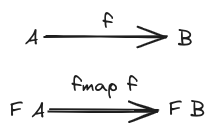
\includegraphics[width=0.3\textwidth]{figs/functor}
    \end{figure}

    \vocab{Контравариантный функтор} --- пара из типового конструктора и операции на функциях, разворачивающей стрелку.
    Плюс соответствующие законы.

    \begin{minted}{haskell}
        class Contravariant f where
          contramap :: (a -> b) -> (f b -> f a)
    \end{minted}

    \begin{figure}[H]
        \centering
        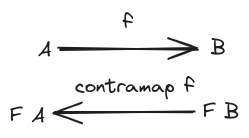
\includegraphics[width=0.3\textwidth]{figs/contra-functor}
    \end{figure}

    Типовой конструктор можно объявить ковариантным или контравариантным функтором (или никаким из них) относительно типового параметра в зависимости от вида декларации соответствующих конструкторов данных.
    А именно, от \vocab{полярности}\footnote{\url{https://existentialtype.wordpress.com/2012/08/25/polarity-in-type-theory/}}\footnote{\url{https://ncatlab.org/nlab/show/polarity+in+type+theory}} позиций, в которых входит этот типовой параметр в декларации.

    Попробуем развить интуитивное понимание полярностей.
    Рассмотрим некоторое вычисление типа \texttt{F a}.
    Параметр \texttt{a} входит в положительной позиции, если все его значения можно извлечь из \texttt{F a}, как в следующих примерах (для извлечения могут понадобиться паттерн-матчинг и аппликация):
    \begin{minted}{haskell}
        data F a = L a | R a
        data F a = D a (Int -> a)
    \end{minted}

    Вхождения, наоборот, отрицательные, если значения соответствующего типа нельзя получить из вычисления, но нужно ему предоставить.
    Например, в качестве параметров функций:
    \begin{minted}{haskell}
        data F a = F (a -> Int)
        data F a = L (a -> ()) | R Int
    \end{minted}
    Действительно, для первого примера можно объявить инстанс \mintinline{haskell}|Contravariant|:
    \begin{minted}{haskell}
        instance Contravariant F where
          contramap :: (a -> b) -> (F b -> F a)
          contramap g (F f) = F (f . g)
    \end{minted}

    Можно предположить, что на плюс и минус действуют обычные мультипликативные законы.
    И это действительно так.
    \begin{itemize}
        \item Плюс на плюс даёт плюс:
        \begin{minted}{haskell}
            data F a = F (Int -> (Int -> a))
        \end{minted}
        \item Плюс на минус (и наоборот) --- минус:
        \begin{minted}{haskell}
            data F a = F ((Int -> a) -> Int)
        \end{minted}
        \item Минус на минус --- плюс, поскольку параметр принимаемой функции выдаётся реализацией вызывающей стороне:
        \begin{minted}{haskell}
            data F a = F ((a -> Int) -> Int)
        \end{minted}
    \end{itemize}

    Тип от двух положительных параметров можно объявить \vocab{бифунктором}:
    \begin{minted}{haskell}
        class Bifunctor f where
          bimap :: (a -> c) -> (b -> d) -> f a b -> f c d
    \end{minted}

    Тип от двух параметров, положительного и отрицательного, --- \vocab{профунктором}:
    \begin{minted}{haskell}
        class Profunctor p where
          dimap :: (c -> a) -> (b -> d) -> p a b -> p c d
    \end{minted}

    Профункторы являются некоторыми обобщениями функциональной стрелки.
    Например, если у нас есть SQL запрос, который по данным возвращает результат, его можно объявить профунктором с семантикой --- добавить пред-обработку входных данных и пост-обработку выходных:
    \begin{minted}{haskell}
        dimap serialize deserialize (query :: Text -> Text) :: Age -> [User]
    \end{minted}

    Также понятие вариантности часто встречается в объектно ориентированных языках для обозначения возможности дополнить отношение подтипизации на полиморфные типы (да и вообще в теории подтипизации).

    Действительно, \vocab{отношение подтипизации} \texttt{B <: A} говорит о том, что значение типа \texttt{B} безопасно использовать в позиции, где ожидается значение типа \texttt{A}.
    Иначе говоря, существует функция \texttt{upcast :: B -> A}.
    Если типовой конструктор \texttt{F a} ковариантен относительно параметра \texttt{a}, то по \texttt{upcast} найдётся \texttt{upcast' :: F B -> F A}.
    То есть отношение подтипизации также автоматически включает \texttt{F B <: F A}.
    Контравариантный случай аналогично.

    \begin{task}
        Убедитесь в вашем любимом языке с поддержкой вариантности, что минус на минус даёт плюс.
    \end{task}

    \subsubsection{Data promotion \& kind polymorphism} \label{subsubsec:promotion}

    Ранее мы программировали на уровне термов, а типы контролировали ``правильность'' построения термов.
    Но типы так же являются языком как с синтаксической точки зрения, так и с вычислительной.
    Вычисления на типах мы будем рассматривать далее, а в этом параграфе научимся конструировать в Haskell различные структуры на уровне типов.

    В качестве модельной задачи зададим структуру данных, моделирующую вектор, но такую, что тип будет параметризован длиной.
    Для начала определим натуральные числа на уровне типов в стиле Пеано:
    \begin{minted}{haskell}
        data Zero
        data Suc n
    \end{minted}

    \begin{task}
        Сколько обитателей типа \mintinline{haskell}|Suc (Suc Zero)|?
    \end{task}

    Теперь мы можем задать тип вектора, содержащий информацию о длине:
    \begin{minted}{haskell}
        data Vec (size :: Type) (elem :: Type) where
          VNil :: Vec Zero a
          VCons :: a -> Vec n a -> Vec (Suc n) a

        example :: Vec (Suc (Suc Zero)) Int
        example = VCons 1 (VCons 2 VNil)
    \end{minted}

    Для такого типа, например, можно написать безопасную функцию \mintinline{haskell}|zip|, работающую только на векторах одинаковой длины:
    \begin{minted}{haskell}
        vzip :: Vec n a -> Vec n b -> Vec n (a, b)
        vzip VNil VNil = VNil                                      -- n ?$\sim$? Zero
        vzip (VCons x xs) (VCons y ys) = VCons (x, y) (vzip xs ys) -- n ?$\sim$? Suc n'
    \end{minted}

    Заметьте, что в остальных ветках \mintinline{haskell}|vzip| должны возникнуть эквивалентности, начинающиеся с различных конструкторов, например, \mintinline{haskell}|Zero ?$\sim$? Suc n|.
    Поскольку невозможно построить такие аргументы функции, Haskell позволяет соответствующие ветки не рассматривать.

    \begin{task}
        Напишите функцию добавления в конец элемента вектора.
        Двигайтесь последовательно, заполняя типовые дыры и отслеживая возникающие эквивалентности.
    \end{task}

    Удивительно, но сейчас наш язык типов не типизирован.
    Действительно, кайнд \mintinline{haskell}|Suc| --- \mintinline{haskell}|Suc :: Type -> Type|, соответственно ничто не мешает написать \mintinline{haskell}|Suc (Maybe Int)|.
    То есть язык кайндов, который должен контролировать типы, слишком беден.
    В то же время он слишком ограничивающий, поскольку не поддерживает полиморфизм, что дало начало большому количеству дублирований а ля \mintinline{haskell}|Typeable (ty :: Type)|, \mintinline{haskell}|Typeable1 (ty :: Type -> Type)|\ldots

    Чтобы обогатить систему кайндов для лучшего контроля за программами уровня типов, System $F_C$ была расширена до System $F_C^\uparrow$ (читается FC-pro)~\cite{yorgey2012giving}.
    Это достигается автоматическим продвижением (promotion) \mintinline{haskell}|data| деклараций на уровень выше (расширение \href{https://downloads.haskell.org/ghc/latest/docs/users_guide/exts/data_kinds.html#extension-DataKinds}{DataKinds}).
    А именно: любой конструктор типа также становится кайндом, а конструктор данных --- конструктором типа.
    Так, в примере с числами, мы можем задекларировать натуральные числа как обычно и использовать на уровне типов:
    \begin{minted}{haskell}
        data Nat = Zero | Suc Nat
        ghci> :k Suc :: Nat -> Nat
    \end{minted}

    Теперь вектору можно приписать более точный кайнд:
    \begin{minted}{haskell}
        data Vec (size :: Nat) (elem :: Type) where
          VNil :: Vec Zero a
          VCons :: a -> Vec n a -> Vec (Suc n) a
    \end{minted}

    \begin{task}
        Что выведет \mintinline{haskell}|ghci> :k Vec|?
    \end{task}

    Поскольку типы и термы в Haskell живут в разных пространствах имён, можно называть конструкторы типов и данных одинаково.
    Однако если продвинуть такой тип данных, возникнет неоднозначность: мы имеем в виду тип или продвинутый конструктор.
    Haskell позволяет указать явно, что речь идёт о продвинутом конструкторе с помощью одинарной кавычки.
    \begin{minted}{haskell}
        data T = T Nat
        ghci> :k T
        T :: Type      -- Речь про конструктор типа
        ghci> :k 'T
        'T :: Nat -> T -- Речь про продвинутый конструктор данных
    \end{minted}

    Недавние версии GHC поддерживают прямое объявление конструкций уровня типов с помощью расширения \href{https://downloads.haskell.org/ghc/latest/docs/users_guide/exts/type_data.html#extension-TypeData}{TypeData}.
    Не любые \mintinline{haskell}|data| декларации подходят для продвижения, в то же время \mintinline{haskell}|type data| декларации позволяют явно запросить структуру уровня типов и получить внятные ошибки, если декларация написана неправильно.
    \begin{minted}{haskell}
        type data Nat = Zero | Suc Nat
    \end{minted}

    В случае продвижения полиморфного типа, мы получаем полиморфные кайнды (\href{https://downloads.haskell.org/ghc/latest/docs/users_guide/exts/poly_kinds.html}{PolyKinds}):
    \begin{minted}{haskell}
        data [a] = [] | (:) a [a]
        ghci> :k '(:)
        '(:) :: forall k . k -> [k] -> [k]
    \end{minted}

    \begin{figure}
        \centering
        %! suppress = Quote
        \begin{tabular}{|c|c|c|}
            \hline
            Term                                   & Type                                            & Kind                                            \\
            \hline
            \mintinline{haskell}|Zero|             & \mintinline{haskell}|Nat|                       & \mintinline{haskell}|Type|                      \\
            \mintinline{haskell}|[Zero, Suc Zero]| & \mintinline{haskell}|[Nat]|                     & \mintinline{haskell}|Type|                      \\
            \mintinline{haskell}|[]|               & \mintinline{haskell}|forall a. [a]|             & \mintinline{haskell}|Type|                      \\
            \mintinline{haskell}|(:)|              & \mintinline{haskell}|forall a. a -> [a] -> [a]| & \mintinline{haskell}|Type|                      \\
            & \mintinline{haskell}|'Suc 'Zero|                & \mintinline{haskell}|Nat|                       \\
            & \mintinline{haskell}|'['Zero, 'Suc 'Zero]|      & \mintinline{haskell}|[Nat]|                     \\
            & \mintinline{haskell}|'[Int, Double]|            & \mintinline{haskell}|[Type]|                    \\
            & \mintinline{haskell}|'[]|                       & \mintinline{haskell}|forall k. [k]|             \\
            & \mintinline{haskell}|'(:)|                      & \mintinline{haskell}|forall k. k -> [k] -> [k]| \\
            \hline
        \end{tabular}
        \caption{Пример вселенных в Haskell.}
        \label{fig:universes}
    \end{figure}

    Примеры продвижения различных конструкций можно увидеть в таблице~\ref{fig:universes}.

    Зададим гетерогенный список, индексированный типами элементов:
    \begin{minted}{haskell}
        data HList (tys :: [Type]) where
          HNil :: HList '[]
          HCons :: ty -> HList tys -> HList (ty ': tys)

        example :: HList '[Int, Bool, Double]
        example = HCons 42 $ HCons True $ HCons 12.5 HNil
    \end{minted}

    Структуры данных тоже могут быть полиморфными по кайндам.
    Рассмотрим следующий тип \href{https://hackage.haskell.org/package/tagged-0.8.8/docs/Data-Tagged.html#t:Tagged}{\mintinline{haskell}|Tagged|}, позволяющий дополнить тип значения дополнительным типовым тегом.
    Кайнд тега может быть произвольным, поэтому, например, можем использовать встроенные в систему типов константы \href{https://ghc.gitlab.haskell.org/ghc/doc/users_guide/exts/type_literals.html}{TypeLits}:
    \begin{minted}{haskell}
        newtype Tagged (tag :: k) (a :: Type) = Tagged a
        ghci> :t Tagged
        Tagged :: forall k (tag :: k) a. a -> Tagged tag a

        example :: Tagged ("hello" :: Symbol) Int
        example = Tagged 42
    \end{minted}

    Современный Haskell в итоге пришёл к тому, что система типов не делает различий между типами и кайндами (рис.~\ref{fig:types-eq-kinds}).
    В частности, \mintinline{haskell}|Type :: Type|.
    Это нужно для расширения возможностей Haskell в сторону программирования с зависимыми типами путём добавления несинтаксических эквивалентностей для кайндов (\href{https://ghc.gitlab.haskell.org/ghc/doc/users_guide/exts/poly_kinds.html#extension-TypeInType}{TypeInType}).
    $System~FC$ была представлена в работе~\cite{weirich2013system}\footnote{\href{https://www.youtube.com/watch?v=ISGENChlA4M&list=PLvPsfYrGz3wufQguebnCduYgQQ9UMeJRt}{(youtube) Мини-курс на русском языке про развитие Haskell в сторону зависимой типизации.}}\footnote{\href{https://www.youtube.com/watch?v=_HYI7zjkrEs&list=PLvPsfYrGz3wuVAGhNf6-i7uafXg56oqM5&index=1}{(youtube) Мини-курс на русском языке --- система вывода типов Haskell.}}.

    \begin{figure}
        \centering
        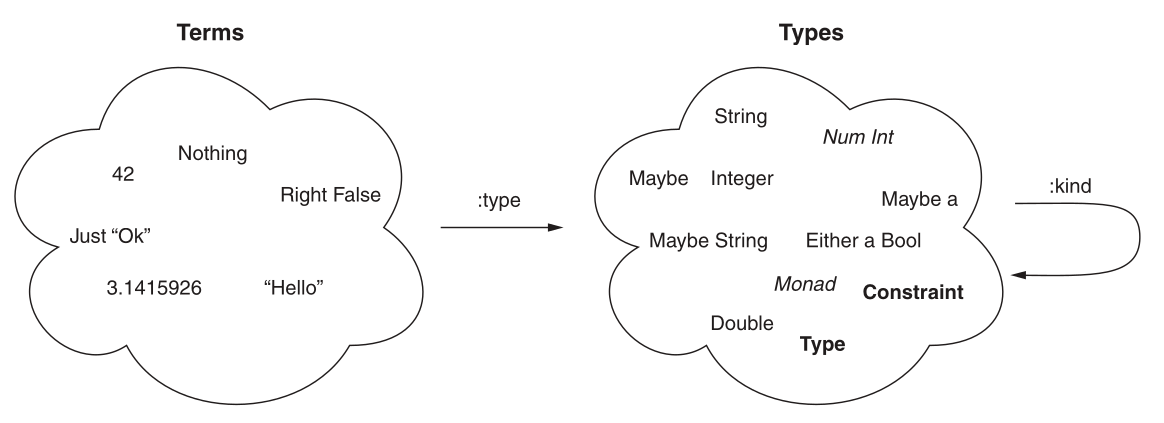
\includegraphics[width=0.99\textwidth]{figs/types-eq-kinds}
        \caption{Типы и канды --- одно~\cite{bragilevsky-haskell}.}
        \label{fig:types-eq-kinds}
    \end{figure}

    \subsection{Реализация параметрического полиморфизма}

    \vocab{Конвенция вызова}\footnote{\url{https://en.wikipedia.org/wiki/Calling_convention}} представляет собой набор соглашений между тем, как функция компилируется и как должна вызываться.
    Например, функция принимает два аргумента, каждый размером в машинное слово, и возвращает один результат размером в машинное слово.
    Тогда сгенерированный низкоуровневый код этой функции может, например, ожидать, что оба аргумента передаются через специальную пару регистров, а складывать результат он будет в третий.
    В таком случае вызывающий код обязан предоставить аргументы в правильных регистрах и ожидать результата в некотором третьем, заранее оговоренном регистре.

    В общем случае, конвенция вызова функции зависит от типов аргументов и результата.
    Нужно знать как минимум их размер, чтобы понять, размещать их в регистрах или на стеке.
    Нужно знать, это указатель или значение само по себе, чтобы понимать, как с ним работать.

    Таким образом, реализация параметрического полиморфизма в языке --- это не тривиальная задача.
    Разные языки используют различные подходы, все со своими достоинствами и недостатками.

    \subsubsection{Mономорфизация} \label{subsubsec:monomorphization}

    \vocab{Mономорфизация} --- самый прямолинейный подход, компилируем функцию отдельно для каждого набора типовых аргументов.
    Так, если различных наборов типовых аргументов, с которыми эта функция вызывается, например, 100 (что запросто может быть), то её код будет компилироваться сто раз и занимать в бинарнике в сто раз больше места.
    Так делают, например, C++ и Rust.

    На самом деле всё ещё хуже.
    Если проект многомодульный и состоит из множества единиц компиляции (кусков, которые компилируются отдельно), то одна и та же специализация функции на типовые аргументы будет компилироваться заново во всех единицах компиляции, где такая специализация нужна.
    А затем, линкер будет заниматься удалением дубликатов, что тоже не самый быстрый и эффективный процесс.

    \begin{itemize}
        \item[\positive] Порождаемый код максимально эффективен для каждого типа;
        \item[\negative] Время компиляции крайне велико;
        \item[\negative] Существенно увеличивается размер результирующего бинарного файла, что может быть критично для некоторых приложений;
        \item[\negative] Может неэффективно работать из-за засорения кеша кода в процессоре;
        \item[\negative] В интерфейсах не может быть полиморфных методов, так как мы не знаем в месте вызова, к какому именно наследнику относится вызываемый метод, и какой код нужно специализировать;
        \item[\negative] К полиморфным функциям нельзя динамически линковаться (у них нет кода до специализации);
        \item[\negative] Нельзя поддержать variance, потому что код компилируется для конкретного типа и в общем случае не может работать для произвольного подтипа или супертипа.
    \end{itemize}

    Некоторые языки не делают инстанциацию скрытой деталью реализации языка, а предоставляют её как инструмент пользователям.
    Так делают, например, C++ и Zig.
    А именно, это позволяет добиться следующего:
    \begin{itemize}
        \item Если разрешить использовать значения в типах, инстанциация может использоваться как механизм вычислений на этапе компиляции.
        \item Если отложить проверку ошибок на стадию инстанциирования, то мы получим своего рода статическую утиную типизацию.
        Это позволит не описывать сложные сигнатуры полиморфных функций.
        Однако тогда функции придётся вручную инстанциировать против всевозможных типов, иначе нельзя понять статически, компилируется она хотя бы против этих типов или нет.
    \end{itemize}

    \subsubsection{Стирание типа} \label{subsubsec:type-erasure}

    Можно всё сделать наоборот, унифицировав значения, которые приходят на вход полиморфным функциям, вместо того, чтобы компилировать код под каждый тип.

    Пусть каждое значение будет аллоцировано в куче и передаваться по указателю.
    Тогда мы сможем переиспользовать один и тот же код для разных типовых аргументов, он просто будет ожидать указатели.

    \begin{itemize}
        \item[\positive] Каждая функция компилируется ровно один раз --- быстро;
        \item[\positive] Можно динамически загружать новые полиморфные функции и типы и использовать их друг с другом;
        \item[\positive] Гибкость --- вариантность, полиморфные методы в интерфейсах, higher-ranked types\ldots просто работают;
        \item[\negative] Аллокация в куче и разыменование указателя может очень сильно замедлить код, особенно работающий с ``примитивными типами'';
        \item[\negative] Поскольку информация о типах стирается, нельзя ничего сделать с типовым аргументом, не имея его обитателей (например, запросить рефлексией информацию).
    \end{itemize}

    Такого подхода придерживаются JVM, Haskell и, как правило, другие функциональные языки ввиду его гибкости.

    Особую проблему вызывает работа с примитивами, потому что каждое значение приходится сначала боксить (переносить в кучу), а потом уже использовать в полиморфном контексте.
    Поэтому языки борются с этим как могут.
    Некоторые языки урезают диапазоны значений примитивов, чтобы зарезервировать бит, определяющий, это указатель или значение.
    Код консультируется с этим битом для работы (похоже на~\ref{subsubsec:swift-generics}).
    Так делают, например, OCaml и \href{https://koka-lang.github.io/koka/doc/book.html#sec-value-types}{Koka}.
    Агрессивный инлайнинг тоже помогает.
    Java пытается аккуратно двигаться в сторону возможности мономорфизации\footnote{\href{https://youtu.be/JI09cs2yUgY?si=MLkRs31mN1koXIu1}{Type Specialization of Java Generics - What If Casts Have Teeth ?}}\footnote{\url{https://cr.openjdk.org/~jrose/values/parametric-vm.html}}.

    \subsubsection{Гибридный подход} \label{subsubsec:hybrid}

    С\# реализует гибридный подход\footnote{\href{https://learn.microsoft.com/en-us/dotnet/csharp/programming-guide/generics/generics-in-the-run-time}{Generics in the runtime (C\# programming guide).}}.
    Они различают значения, хранимые в куче --- \vocab{reference types}, и значения, хранимые на стеке --- \vocab{value types}.
    Для первых они генерируют одну специализацию, работающую с указателями.
    Для каждого набора value-типов они генерируют лениво в рантайме специализацию.

    То есть следы дженериков в таком подходе есть в промежуточном представлении CIL, а также в рантайме.

    \begin{itemize}
        \item[\positive] Порождается эффективный код, работающий с примитивами;
        \item[\positive] Доступна рефлексия по дженерикам;
        \item[\positive] Небольшое время компиляции;
        \item[\negative] Инстанциация в рантайме замедляет исполнение;
        \item[\negative] Variance работает только для reference types (что странно --- есть ``правильная'' подтипизация, а есть ``неправильная'').
    \end{itemize}

    % todo выпросить инфу про подтипизацию у Михаила

    \subsubsection{Использование виртуальной таблицы свойств типов} \label{subsubsec:swift-generics}

    Swift\footnote{\href{https://youtu.be/ctS8FzqcRug?si=y_ZYnuUOulA33d_X}{2017 LLVM Developers’ Meeting: ``Implementing Swift Generics''}} вместе с каждым типовым параметром передаёт value witness table (рис.~\ref{fig:swift-witness-table}).
    Это таблица со всей необходимой информацией, о типе: размер и выравнивание, что нужно сделать при копировании и перемещении объекта (например, инкрементировать счётчик ссылок).
    Таким образом, скомпилированный код постоянно обращается к этой таблице и делает виртуальные вызовы функций из неё (рис.~\ref{fig:swift-generated-code}).
    \begin{figure}
        \centering
        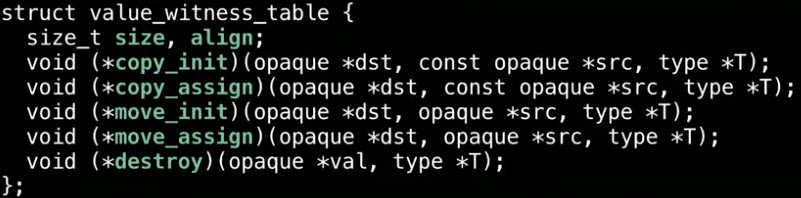
\includegraphics[width=0.7\textwidth]{figs/swift-witness-table}
        \caption{Swift value witness table.}
        \label{fig:swift-witness-table}
    \end{figure}
    \begin{figure}
        \centering
        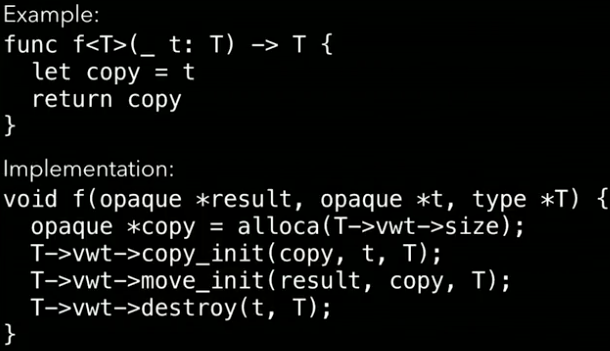
\includegraphics[width=0.6\textwidth]{figs/swift-generated-code}
        \caption{Код полиморфной функции, порождаемый компилятором Swift.}
        \label{fig:swift-generated-code}
    \end{figure}

    \begin{itemize}
        \item[\positive] Небольшое время компиляции;
        \item[\positive] Предсказуемая эффективность (не приводит к неожиданным паузам в рантайме);
        \item[\positive] Эффективная работа с value-значениями;
        \item[\positive] Высокая гибкость;
        \item[\positive] Информация о типах не стирается;
        \item[\negative] Серьёзный константный оверхед на динамические вызовы через таблицу, эффективность очень сильно зависит от компиляторных оптимизаций.
    \end{itemize}

    Своего рода реализация параметрического полиморфизма через специальный.

    \subsection{Полиморфизм по конвенции вызова} \label{subsec:representation-polymorphism}

    Как мы уже обсуждали выше~\ref{subsubsec:type-erasure}, параметрический полиморфизм в Haskell реализуется следующим образом: все значения хранятся в куче и передаются в полиморфные функции по указателю.
    Однако, если для вычислительного кода важна производительность, такой подход не годится ввиду большой нагрузки на подсистему управления памятью и множества индирекций.
    Поэтому Haskell позволяет также писать код с использованием unboxed значений.
    А если конвенция вызова не принципиальна, можно по ней абстрагироваться и писать один код для boxed и unboxed значений~\cite{eisenberg2017levity}.

    \subsubsection{Классификация значений по runtime представлению}

    \begin{figure}
        \centering
        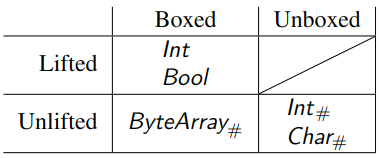
\includegraphics[width=0.5\textwidth]{figs/haskell-value-kinds}
        \caption{Виды значений в Haskell с примерами~\cite{eisenberg2017levity}.}
        \label{fig:haskell-value-kinds}
    \end{figure}

    На рисунке~\ref{fig:haskell-value-kinds} можно увидеть классификацию значений в Haskell с примерами типов.
    \vocab{Unboxed типы} --- их значения удерживаются и передаются по значению.
    \vocab{Boxed}, соответственно, наоборот, передаются по указателю и хранятся в куче.
    Обычный \mintinline{haskell}|Int| является просто декларацией следующего вида, где \mintinline{haskell}|I#| --- это обычный конструктор с необычным именем, содержащий unboxed значение.
    \begin{minted}{haskell}
        data Int = I# Int#
    \end{minted}

    \vocab{Lifted типы} --- содержат $\bot$ в качестве значения.
    Иначе говоря, могут содержать отложенные вычисления.
    \vocab{Unlifted типы} --- наоборот, не могут быть отложенными.
    Операции, производящие значения unlifted типов всегда энергичные.
    Свойство lifted/unlifted называют \vocab{levity}.
    Чтобы распространить дальнейшее изложение на энергичные языки, можно levity заменить на boxity и всё останется справедливым.

    \# в именах типов и функций --- это конвенция, показывающая, что где-то рядом происходит работа с unlifted значениями\footnote{Нужно подключить расширение \href{https://ghc.gitlab.haskell.org/ghc/doc/users_guide/exts/magic_hash.html}{MagicHash}, чтобы пользоваться \# в идентификаторах.}.

    Также в Haskell есть unboxed кортежи, которых не существует на этапе исполнения.
    Например, следующая функция как бы возвращает пару значений, но в действительности компилятор может их разместить, например, в паре регистров.
    Соответственно, паттерн-матчинг по таким кортежам, просто позволяет сослаться на каждое из этих значений.
    \begin{minted}{haskell}
        divMod# :: Int -> Int -> (# Int, Int #)
        case divMod# n k of (# quot, rem #) -> ...
    \end{minted}
    Соответственно, нет никакого различия между по-разному вложенными unboxed кортежами:
    \begin{minted}{haskell}
        (# A, (# B, C #)) ?$\equiv$? (# #( A, B #), C #) ?$\equiv$? (# A, B, C #)
    \end{minted}

    \subsubsection{Representation polymorphism}

    Значения различных типов могут быть на этапе исполнения устроены по-разному.
    То есть нам нужна некоторая система классификации типов.
    Но такая система в Haskell уж есть --- кайнды.
    Опишем в виде структур данных предметную область, а потом продвинем на нужный уровень с помощью DataKinds~\ref{subsubsec:promotion}.

    Стандартная библиотека Haskell \href{https://downloads.haskell.org/ghc/latest/docs/users_guide/exts/representation_polymorphism.html}{предоставляет} следующие типы данных:
    \begin{minted}{haskell}
        TYPE :: RuntimeRep -> Type

        data Levity = Lifted | Unlifted

        data RuntimeRep = BoxedRep Levity
                        | IntRep | DoubleRep
                        | TupleRep [RuntimeRep]
                        | SumRep [RuntimeRep]
                        | ...

        type LiftedRep = BoxedRep Lifted

        type Type = TYPE LiftedRep
    \end{minted}

    \mintinline{haskell}|TYPE| --- это магический тип, определённый в компиляторе.
    Он параметризован runtime-представлением значений.
    Теперь привычный \mintinline{haskell}|Type| --- это частный случай с boxed lifted значениями.

    \begin{itemize}
        \item \mintinline{haskell}|Int :: TYPE (BoxedRep Lifted)| или \mintinline{haskell}|:: Type|
        \item \mintinline{haskell}|IntRep| и \mintinline{haskell}|DoubleRep| соответствуют представлению численных констант (в зависимости от архитектуры процессора, целые числа и числа с плавающей запятой может быть необходимо располагать в различных специальных регистрах)\\ \mintinline{haskell}|Int# :: TYPE IntRep|
        \item \mintinline{haskell}|Maybe Int :: Type|
        \item \mintinline{haskell}|Maybe :: Type -> Type|
        \item \mintinline{haskell}|TupleRep| и \mintinline{haskell}|SumRep| --- unboxed алгебраические типы, представления параметризованы представлениями хранимых значений\\
        \mintinline{haskell}|(# Int, Bool #) :: TYPE (TupleRep '[LiftedRep, LiftedRep])|
        \item Для простоты не унифицируются типы вложенных кортежей
        \begin{minted}{haskell}
            (# Int#, (# Int, Double# #) #)
              :: TYPE (TupleRep '[IntRep, TupleRep '[LiftedRep, DoubleRep]])
        \end{minted}
    \end{itemize}

    Выставив runtime-представление в структуре кайндов, мы теперь можем параметризоваться по ним.
    Например, кайнд функциональной стрелки выглядит следующим образом\footnote{Выключить упрощения: \mintinline{haskell}|ghci> :set -fprint-explicit-foralls -fprint-explicit-runtime-reps|}:
    \begin{minted}{haskell}
        ghci> :k (->)
        (->) :: forall {q :: RuntimeRep} {r :: RuntimeRep}. TYPE q -> TYPE r -> Type
    \end{minted}

    К сожалению, Haskell выставляет довольно строгое ограничение: связыватели не могут иметь тип, полиморфный по runtime представлению.
    Можно легко предположить, почему, --- нельзя сгенерировать код функции для работы с параметром произвольного рантайм-представления.
    Это можно решить только мономорфизацией~\ref{subsubsec:monomorphization}, но Haskell избегает этого подхода\footnote{\url{https://gitlab.haskell.org/ghc/ghc/-/issues/14917}}.
    Сообщество также пытается найти другие решения\footnote{\url{https://mail.haskell.org/pipermail/haskell-cafe/2023-January/135770.html}} (что-то вроде~\ref{subsubsec:swift-generics}).

    Например, изначально оператор аппликации был обобщён только по возвращаемому типу.
    Это не порождает проблем, так как вызывающий код сможет вывести представление и сгенерировать подходящий код:
    \begin{minted}{haskell}
        ($) :: forall r a (b :: TYPE r). (a -> b) -> a -> b
        f $ ?\framebox{x}? = f x
    \end{minted}

    Однако, было замечено, что для оператора аппликации можно получить другую реализацию, не использующую levity-полиморфное связывание\footnote{\url{https://gitlab.haskell.org/ghc/ghc/-/merge_requests/10131}}:
    \begin{minted}{haskell}
        ($) :: forall ra rb (a :: TYPE ra) (b :: TYPE rb). (a -> b) -> a -> b
        ($) f = f
    \end{minted}


    \clearpage


    \section{Специальный полиморфизм} \label{sec:ad-hoc}





    \cite{hudak2007history}

    \cite{wadler1989make}

    % todo what do you want to give name to

    % todo implicit parameters

    % todo constraint is a proposition and dict is a proof

    % todo constraints package of Edward Kmett

    % todo monomorphism restriction

    % todo pattern-matching on types

    % todo serializer and serializable

    % todo proxy

    % todo algebra driven design

    % todo rules and coersion

    % todo type classes vs interfaces
    % todo type classes via interfaces and implicits

    % todo incoherent instances

    % todo instance arguments

    % todo Monoid a => Monad m ??

    % todo https://downloads.haskell.org/ghc/latest/docs/users_guide/exts/constraints.html

    % todo ConstraintKinds

    % todo constraints and decidability

    % todo https://chrisdone.com/posts/haskell-constraint-trick/

    % todo A Reflection on Types SPJ paper

    % todo haskell specialization

    % todo https://wiki.haskell.org/Inlining_and_Specialisation

    % todo existential types, different vtable implementations, value types support
    % todo scala type classes
    % todo type inhabitation, system FC, Symon's talk
    % todo доклад SPJ
    % todo open unions, data a la carte
    % todo roles and coertions
    % todo typeable & reflection
    % todo reflecrtion https://www.tweag.io/blog/2017-12-21-reflection-tutorial/
    % todo How to make ad-hoc polymorphism less ad-hoc

    % todo C. V. Hall, K. Hammond, S. L. Peyton Jones, and P. L. Wadler. Type classes in haskell

    % todo S. Peyton Jones, S. Weirich, R. A. Eisenberg, and D. Vytiniotis. A reflection on types. In A list of successes that can change the world,

    % todo \chapter*{"Hackett: a metaprogrammable Haskell" by Alexis King}

    % todo

    \cite{constraint-kind}

    % todo call stack

    % todo примеры с HList

    % todo orphans

    Для GHC можно указать правила переписывания, которые заставят компилятор использовать специализированные версии для определённых типов\footnote{\href{https://downloads.haskell.org/~ghc/6.12.2/docs/html/users\_guide/rewrite-rules.html\#rule-spec}{GHC user guide. Rewrite rules. Specialization.}}.
    \begin{minted}{haskell}
        {-# RULES "genericLookup/Int" genericLookup = intLookup #-}
    \end{minted}

    % todo functional dependencies & associated types

    % todo https://downloads.haskell.org/~ghc/9.0.1/docs/html/users_guide/exts/constraints.html

    % todo Orphan rules

    % todo builder code serialization format from babylon

    % todo associated type families

    % todo reference dependent types

    % todo рулесы, законы и оптимизация

    % todo asking to fill parameters for you because they are very obvious. Implicit in dependently-typed languages

    % todo variadics, open sums and products

    % todo


    \section{Продолжения (continuations)} \label{sec:continuations}

    % todo

    % todo связь с монадами

    % todo монада Cont

    % todo delimited continuations

    % todo sicp

    % todo raynolds The Discoveries of Continuations

    % todo correspondence to negation in intuitionistic logic?

    % todo CPS correspond to double negation in logic reynolds1998definitional

    % todo defuctionalized continuations, pepers from gibbons talk

    % todo difference lists

    % todo he Essence of Cornpiling with Continuations

    % todo calculating correct compilers

    % todo reference to best refactoring
    % todo refrence co calculate correct compilers and stuff

    % todo somedoby's PHD

    \cite{reynolds1972definitional, reynolds1998definitional, defunctionalization-slides}

    % todo jeremy gibbons papers, review the talk

    % todo delimited via undelimited and mutable cell

    % todo transducers, pipelines and internal iteration

    % todo Delimited continuations and asynchronous exceptions

    % todo reason isomorphically


    \section{Интерпретаторы зазеркалья} \label{sec:wonder-interpreters}

    % todo are custom patretns in haskell connected to this?

    % todo initial and final - isomorphism proof

    % todo теоретические основы

    % todo church encoding

    % todo Tagless-final интерпретаторы

    % todo codata, pattern-matching
    % todo custom patterns

    % todo fusion и дефорестация
    % todo haskell inlining
    % todo RULES
    % todo Oleg about fusion and streams
    % todo fused effects

    % todo Reading circle about fusion
    % todo short cut to deforestation
    % todo stream fusion from lists to streams to nothing at all
    % todo call-pattern specialization for Haskell programs

    % todo наверное после континуэйшенов

    % todo композиционность и её восстановление через эксплицирование контекстных зывисимостей.

    % todo threaded code

    % todo connections to polarity https://ncatlab.org/nlab/show/polarity+in+type+theory

    % todo https://okmij.org/ftp/tagless-final/course/Boehm-Berarducci.html

    \cite{gibbons2013functional, gibbons2014folding}

    % todo


    \section{Метапрограммирование и специализация}

    % todo type data GHC extension & datatype promotion

    % todo split intro several topics

    % todo specilization, deforestation, metaprogramming
    % todo staged programming
    % todo modal types for staged programming
    % todo type roles

    % todo streams and fusion
    % todo CPS

    % todo staged computations and modal types
    % todo Haskell papers about fusion

    % todo fist class specialization to beat type families

    % todo generics and Gibbons paper about abstractions
    % todo SOP & variadics

    % todo ghc inlining paper

    % todo https://ora.ox.ac.uk/objects/uuid:cd041aa0-8d69-4f18-bce2-6d75244b69b9/files/m7fd9779b27fcb70ae734e66bcd3ee79f

    % todo Oleg's finally tagless partially evaluated paper

    % todo variadics

    % todo Staging with Class

    % todo hygene macro & dynamic scoping

%    \subsection{Template Haskell}
%
%    % todo порядок на коде для поддержания реификации
%
%    % todo
%
%    \subsection{Рефлексия и реификация}
%
%    % TODO
%
%    \subsection{Zig-generics}
%
%    % todo
%
%    \subsection{GHC.Generics}
%
%    % todo
%
%    \subsection{Uniplate}
%
%    % todo


    \section{Дополнительные главы монад}

    % todo ncatlabs

    % todo Monads and algebras

    % todo оригинальная статья

    % todo monadic reflection
    % todo monadic reflection & direct style (lib from scala)

    % todo free monads, freer monads

    % todo монады не композируются, но фримонады - композируются

    % todo semantic domains have monad structure

    % todo https://github.com/lampepfl/monadic-reflection/blob/main/TUTORIAL.md

    % todo C# expression trees
    % todo F# что-то про монады и forM

    % todo call by push value

    % todo monads in pythong with nice syntax

    % todo lazyness
    % todo direct style

    % todo


    \section{Хендлеры эффектов} \label{sec:effect-handlers}

    % todo monad error is a bullshit

    % todo https://homepages.inf.ed.ac.uk/wadler/papers/expression/expression.txt

    % todo https://www.eff-lang.org/handlers-tutorial.pdf

    % todo алгебраические эффекты
    % todo связь с delimited continuations
    % todo стратегии компиляции, связь с codata
    % todo эффекты высших порядков
    % todo full vs shallow embeddings
    % todo abstracting definitional interpreters & github semantics
    % todo fused effects and CPS

    % todo expression problem

    % todo compare open type families & extensible interpreters

    % todo Polymorphic Symmetric Multiple Dispatch with Variance

    % todo \textit{multimethods}

    % todo  custom schedulers

    Languages with \textit{multimethods}, like Common Lisp’s CLOS, Dylan, and Julia do support adding both new types and operations easily.
    What they typically sacrifice is either static type checking, or separate compilation.

    % todo ZIO, TS Effect


    % todo


    \section{Системы эффектов} \label{sec:effect-systems}

    % todo


    \section{Корутины}

    % todo structured concurrency

    % todo


    \section{Компилятор GHC и runtime}

    % todo Working with Source Plugins paper

    % todo \href{https://gitlab.haskell.org/ghc/ghc/-/wikis/commentary/compiler/generated-code}{\color{blue} I know kung fu: learning STG by example}

    % todo


    \section{Оптика}

    % todo there are pierce lenses

    % todo http://www.timphilipwilliams.com/posts/2019-07-25-minecraft.html

    % todo profunctor optics
    % todo van laarhoven CPS optics

    % todo


    % todo куда-нибудь запихнуть algebra driven design, quick check и доклад про проперти-тесты
    % todo expression problem somewhere
    % todo где-то должно быть содержание книжки про типы Sandy Maguire, data families
    % todo Perhaps Not The Answer You Were Expecting But You Asked For It
    % todo link to SICP

    % todo сказать где-нибудь про вариантность и изоморфизм

    % todo вставить куда-нибудь ссылку на F for Functor

    % todo зависимые типы в Haskell

    % todo где-то нужно про систему кайндов, константы, полиморфизм... Походу Haskell types 101.

    % todo рассовать упражнений по конспекту

    % todo inner and outer iteration - The essence of the iterator pattern

    % todo call-by-push value and how it is related to effects

    % todo Higher-Order Type-Level Programming in Haskell

    % todo как полиморфные кайнды связаны с levity-полиморфизмом

    % todo type families & saturation




    \begin{center}
        \vspace{2em}
        \textit{\LARGE To be continued...}
        \vspace{2em}
    \end{center}


    % todo что-то сделать с порядком
    \newpage
    \bibliography{bib}

\end{document}
